\documentclass[]{tufte-book}

% ams
\usepackage{amssymb,amsmath}

\usepackage{ifxetex,ifluatex}
\usepackage{fixltx2e} % provides \textsubscript
\ifnum 0\ifxetex 1\fi\ifluatex 1\fi=0 % if pdftex
  \usepackage[T1]{fontenc}
  \usepackage[utf8]{inputenc}
\else % if luatex or xelatex
  \makeatletter
  \@ifpackageloaded{fontspec}{}{\usepackage{fontspec}}
  \makeatother
  \defaultfontfeatures{Ligatures=TeX,Scale=MatchLowercase}
  \makeatletter
  \@ifpackageloaded{soul}{
     \renewcommand\allcapsspacing[1]{{\addfontfeature{LetterSpace=15}#1}}
     \renewcommand\smallcapsspacing[1]{{\addfontfeature{LetterSpace=10}#1}}
   }{}
  \makeatother

\fi

% graphix
\usepackage{graphicx}
\setkeys{Gin}{width=\linewidth,totalheight=\textheight,keepaspectratio}

% booktabs
\usepackage{booktabs}

% url
\usepackage{url}

% hyperref
\usepackage{hyperref}

% units.
\usepackage{units}


\setcounter{secnumdepth}{2}

% citations
\usepackage{natbib}
\bibliographystyle{apalike}

% pandoc syntax highlighting
\usepackage{color}
\usepackage{fancyvrb}
\newcommand{\VerbBar}{|}
\newcommand{\VERB}{\Verb[commandchars=\\\{\}]}
\DefineVerbatimEnvironment{Highlighting}{Verbatim}{commandchars=\\\{\}}
% Add ',fontsize=\small' for more characters per line
\newenvironment{Shaded}{}{}
\newcommand{\AlertTok}[1]{\textcolor[rgb]{1.00,0.00,0.00}{\textbf{#1}}}
\newcommand{\AnnotationTok}[1]{\textcolor[rgb]{0.38,0.63,0.69}{\textbf{\textit{#1}}}}
\newcommand{\AttributeTok}[1]{\textcolor[rgb]{0.49,0.56,0.16}{#1}}
\newcommand{\BaseNTok}[1]{\textcolor[rgb]{0.25,0.63,0.44}{#1}}
\newcommand{\BuiltInTok}[1]{#1}
\newcommand{\CharTok}[1]{\textcolor[rgb]{0.25,0.44,0.63}{#1}}
\newcommand{\CommentTok}[1]{\textcolor[rgb]{0.38,0.63,0.69}{\textit{#1}}}
\newcommand{\CommentVarTok}[1]{\textcolor[rgb]{0.38,0.63,0.69}{\textbf{\textit{#1}}}}
\newcommand{\ConstantTok}[1]{\textcolor[rgb]{0.53,0.00,0.00}{#1}}
\newcommand{\ControlFlowTok}[1]{\textcolor[rgb]{0.00,0.44,0.13}{\textbf{#1}}}
\newcommand{\DataTypeTok}[1]{\textcolor[rgb]{0.56,0.13,0.00}{#1}}
\newcommand{\DecValTok}[1]{\textcolor[rgb]{0.25,0.63,0.44}{#1}}
\newcommand{\DocumentationTok}[1]{\textcolor[rgb]{0.73,0.13,0.13}{\textit{#1}}}
\newcommand{\ErrorTok}[1]{\textcolor[rgb]{1.00,0.00,0.00}{\textbf{#1}}}
\newcommand{\ExtensionTok}[1]{#1}
\newcommand{\FloatTok}[1]{\textcolor[rgb]{0.25,0.63,0.44}{#1}}
\newcommand{\FunctionTok}[1]{\textcolor[rgb]{0.02,0.16,0.49}{#1}}
\newcommand{\ImportTok}[1]{#1}
\newcommand{\InformationTok}[1]{\textcolor[rgb]{0.38,0.63,0.69}{\textbf{\textit{#1}}}}
\newcommand{\KeywordTok}[1]{\textcolor[rgb]{0.00,0.44,0.13}{\textbf{#1}}}
\newcommand{\NormalTok}[1]{#1}
\newcommand{\OperatorTok}[1]{\textcolor[rgb]{0.40,0.40,0.40}{#1}}
\newcommand{\OtherTok}[1]{\textcolor[rgb]{0.00,0.44,0.13}{#1}}
\newcommand{\PreprocessorTok}[1]{\textcolor[rgb]{0.74,0.48,0.00}{#1}}
\newcommand{\RegionMarkerTok}[1]{#1}
\newcommand{\SpecialCharTok}[1]{\textcolor[rgb]{0.25,0.44,0.63}{#1}}
\newcommand{\SpecialStringTok}[1]{\textcolor[rgb]{0.73,0.40,0.53}{#1}}
\newcommand{\StringTok}[1]{\textcolor[rgb]{0.25,0.44,0.63}{#1}}
\newcommand{\VariableTok}[1]{\textcolor[rgb]{0.10,0.09,0.49}{#1}}
\newcommand{\VerbatimStringTok}[1]{\textcolor[rgb]{0.25,0.44,0.63}{#1}}
\newcommand{\WarningTok}[1]{\textcolor[rgb]{0.38,0.63,0.69}{\textbf{\textit{#1}}}}

% longtable
\usepackage{longtable,booktabs}

% multiplecol
\usepackage{multicol}

% strikeout
\usepackage[normalem]{ulem}

% morefloats
\usepackage{morefloats}


% tightlist macro required by pandoc >= 1.14
\providecommand{\tightlist}{%
  \setlength{\itemsep}{0pt}\setlength{\parskip}{0pt}}

% title / author / date
\title{Data Visualization in R}
\author{Brooke Anderson}
\date{March 28, 2019}

\usepackage{booktabs}
\usepackage{amsthm}
\usepackage{fontspec}
    \setmainfont{Gill Sans}
\makeatletter
\def\thm@space@setup{%
  \thm@preskip=8pt plus 2pt minus 4pt
  \thm@postskip=\thm@preskip
}
\makeatother

\begin{document}

\maketitle



{
\setcounter{tocdepth}{1}
\tableofcontents
}

\hypertarget{prerequisites}{%
\chapter{Prerequisites}\label{prerequisites}}

\newthought{I have based this workshop} on examples for you to try yourself,
because you
won't be able to learn how to program unless you try it out. I've picked
example data that I hope will be interesting to Navy and Marine Corp public
health researchers and practitioners.

To try out these examples, you need some set-up:

\begin{enumerate}
\def\labelenumi{\arabic{enumi}.}
\tightlist
\item
  Download R
\item
  Download RStudio
\item
  Install some R packages
\item
  Create an R Project for the examples
\item
  Download the example data and save it in the R Project
\end{enumerate}

This section will walk you through each step, explaining both \emph{how} and
\emph{why} to do the step. Click on the \textbf{Next} button (or navigate using the
links at the top of the page) to continue.

\hypertarget{download-r}{%
\section{Download R}\label{download-r}}

\hypertarget{download-rstudio}{%
\section{Download RStudio}\label{download-rstudio}}

\hypertarget{install-some-r-packages}{%
\section{Install some R packages}\label{install-some-r-packages}}

\hypertarget{create-an-r-project}{%
\section{Create an R Project}\label{create-an-r-project}}

\hypertarget{download-example-data}{%
\section{Download example data}\label{download-example-data}}

\hypertarget{plot}{%
\chapter{Plot}\label{plot}}

\newthought{R programming has changed a} lot in the past 10 years or so. This
includes a big
change in the tools used for visualization. The R package \textbf{ggplot2} \citep{R-ggplot2}
is at the heart of one modern style of R visualizations. I'll focus on this style
throughout this workshop, as I think it's an excellent tool for creating
attractive and useful visualizations in a way that is both efficient and easy
to customize (once you get the hang of it).

\hypertarget{plot-elements}{%
\section{Plot elements}\label{plot-elements}}

\newthought{**ggplot2** is based on a} \textbf{grammar of graphics}. To get the hang
of it, you'll need to start thinking of visualizations in terms of separate elements.

\hypertarget{example-data}{%
\subsection{Example data}\label{example-data}}

In my own research, I study the health effects of climate-related disasters, including
heat waves and hurricanes. I noticed that a lot of the sessions at this conference
focus on public health surveillance, so I thought it might be interesting to combine
these two ideas for the example data. On September 10, 2017, Hurricane Irma hit Florida,
and before it did, it triggered evacuations for much of the state. The National Highway
Traffic Safety Administration (under the US Department of Transportation) tracks all
the fatal motor vehicle accidents in the US through its Fatality Analysis Reporting
System (FARS).\footnote{\textbf{Fatality Analysis Reporting System (FARS).} A surveillance system
  for all fatal motor vehicle accidents in the US, maintained by the National Highway
  Traffic Safety Administration. For more, see
  \href{https://www.nhtsa.gov/research-data/fatality-analysis-reporting-system-fars}{the FARS website}.}

I downloaded and cleaned some data from this surveillance system. (In a later section,
I'll tell you more about how to do this cleaning yourself.) I've created a fairly
simple dataset for us to use here. For each date in the weeks around the hurricane's
landfall, it gives the total number of motor vehicle fatalities recorded in the
state. The dataset also gives the week in the year for each date (the first week in
January would be ``1'' for this measure, etc.), as well as the day of the week.
Table \ref{tab:exampledata} shows what this data looks like.

\begin{table}[t]

\caption{\label{tab:exampledata}Number of motor vehicle fatalities in Florida around the date of Hurricane Irma's Florida landfall on September 10, 2017.}
\centering
\begin{tabular}{c|c|c|c}
\hline
Date & Week of year & Day of week & No. of motor vehicle fatalities\\
\hline
2017-08-27 & 35 & Sunday & 4\\
\hline
2017-08-28 & 35 & Monday & 5\\
\hline
2017-08-29 & 35 & Tuesday & 6\\
\hline
2017-08-30 & 35 & Wednesday & 6\\
\hline
2017-08-31 & 35 & Thursday & 6\\
\hline
2017-09-01 & 35 & Friday & 9\\
\hline
2017-09-02 & 35 & Saturday & 8\\
\hline
2017-09-03 & 36 & Sunday & 15\\
\hline
2017-09-04 & 36 & Monday & 7\\
\hline
2017-09-05 & 36 & Tuesday & 8\\
\hline
2017-09-06 & 36 & Wednesday & 7\\
\hline
2017-09-07 & 36 & Thursday & 12\\
\hline
2017-09-08 & 36 & Friday & 9\\
\hline
2017-09-09 & 36 & Saturday & 4\\
\hline
2017-09-10 & 37 & Sunday & 6\\
\hline
2017-09-11 & 37 & Monday & 4\\
\hline
2017-09-12 & 37 & Tuesday & 6\\
\hline
2017-09-13 & 37 & Wednesday & 2\\
\hline
2017-09-14 & 37 & Thursday & 4\\
\hline
2017-09-15 & 37 & Friday & 4\\
\hline
2017-09-16 & 37 & Saturday & 4\\
\hline
2017-09-17 & 38 & Sunday & 10\\
\hline
2017-09-18 & 38 & Monday & 7\\
\hline
2017-09-19 & 38 & Tuesday & 8\\
\hline
2017-09-20 & 38 & Wednesday & 6\\
\hline
2017-09-21 & 38 & Thursday & 5\\
\hline
2017-09-22 & 38 & Friday & 9\\
\hline
2017-09-23 & 38 & Saturday & 7\\
\hline
\end{tabular}
\end{table}

\hypertarget{illustrating-plot-elements}{%
\subsection{Illustrating plot elements}\label{illustrating-plot-elements}}

I've created a simple plot of this data to use to highlight the different
elements of a graph (Figure \ref{fig:plotelements}). This plot shows the
number of motor vehicle fatalities
in Florida per day in the weeks around Hurricane Irma, with the day of the week shown
with color (since, for some health outcomes, there are patterns by the day
of week).

\begin{figure*}
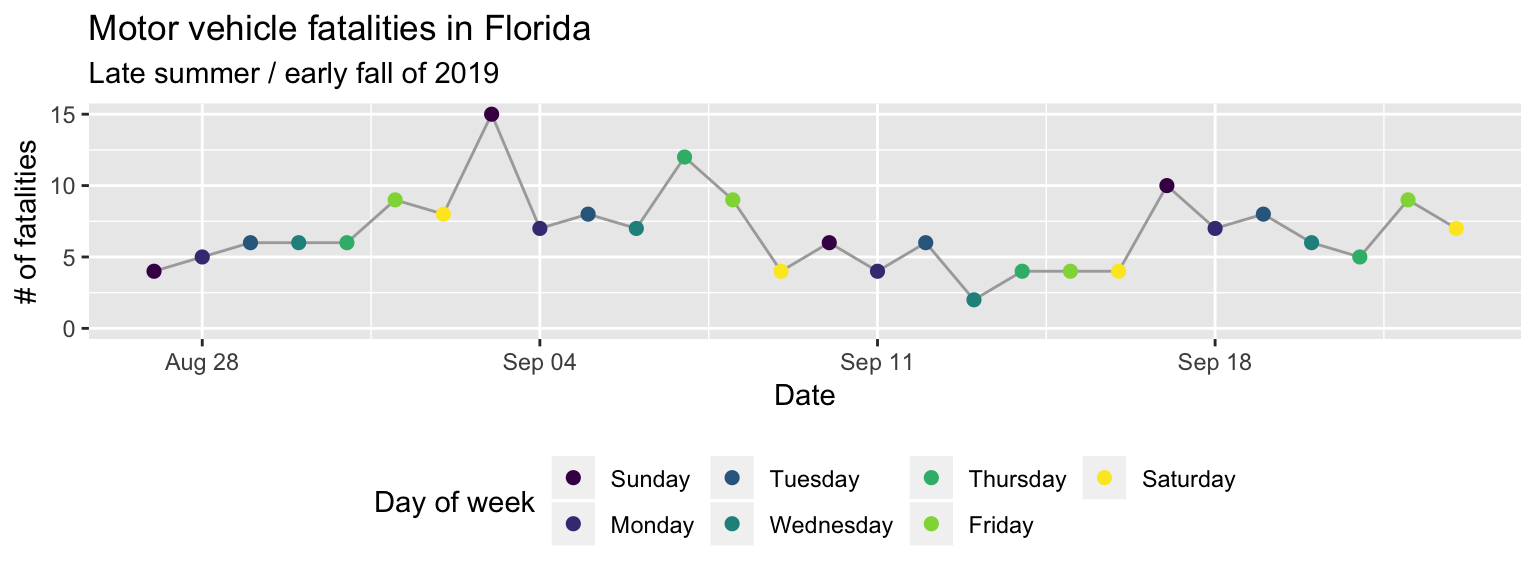
\includegraphics{navy_public_health_files/figure-latex/plotelements-1} \caption[Number of motor vehicle fatalities by day in Florida in the weeks surrounding Hurricane Irma on September 10, 2019]{Number of motor vehicle fatalities by day in Florida in the weeks surrounding Hurricane Irma on September 10, 2019.}\label{fig:plotelements}
\end{figure*}

Let's break this plot into some of its key elements:

\begin{itemize}
\tightlist
\item
  \textbf{data}: The data illustrated with this plot is all from the example data
  shown in Table \ref{tab:exampledata}.
\item
  \textbf{geoms}:\footnote{\textbf{geoms.} The geometric objects (e.g., points, lines, bars, columns,
    polygons, rectangles, text, labels) used to display data for \texttt{ggplot} plots.}
  The geometric objects used to plot the data are (1) points (in
  different colors, depending on the day of week) and (2) a line (in gray).
\item
  \textbf{aesthetics}: For both of the geoms (points and the line), the position along the
  x-axis shows (is \textbf{mapped to}) the date
  given for an observation in the data. The position along the y-axis is mapped to
  the number of fatalities for that observation. For the points (but not the line),
  the color is mapped to the day of week of the observation. For the line, the color
  is always gray (a \textbf{constant aesthetic} for color), rather than color being mapped
  to a value in the data. Other aesthetics---like size, shape, line type and
  transparency---have been left at their default (constant) values.
\item
  \textbf{coordinate system}: The plot uses a \textbf{Cartesian coordinate system}, the most
  common coordinate system you'll use except when creating maps.
\item
  \textbf{scales}: The plot uses a default \textbf{date scale} for the x-axis. For the y-axis,
  the scale is very similar to a default
  \textbf{continuous scale} y-axis, but has been expanded a bit to include 0.
  The \textbf{color scale}is more customized. It uses
  a color scale that's very popular right now called ``viridis'', rather than the
  default color scale.
\item
  \textbf{labels}: This plot uses the axis titles ``Date'' for the x-axis, ``\# of fatalities''
  for the y-axis, and ``Day of week'' for the color scale. In a minute, when you start
  working with the example data, you'll see that these are changed from the corresponding
  column names in the data, to make the plot easier to understand. In addition,
  the plot has both a title (``Motor vehicle fatalities in Florida'') and a
  subtitle (``Late summer / early fall of 2019'').
\item
  \textbf{theme}:\footnote{\textbf{theme.} A collection of specifications for the background elements
    of the plot, including the plot background, grid lines, legend position, text size and
    font, margins, and axis ticks.}
  This plot uses the default \texttt{theme\_gray} theme, with a gray background
  to the main plot area, white gridlines, a Sans Serif font family,
  and a base font size of 11.
  The one customization is that the legend (which here provides the key for
  how color maps to
  day of the week) is shown on the bottom of the plot rather than to the right of
  the plot.
\item
  \textbf{faceting}: This plot does not take advantage of faceting. Instead, the data
  is plotted on a single background. The next example will show an example
  of faceting based on a characteristic of the data.
\end{itemize}

To help the meaning of these elements sink in, Figure \ref{fig:plotelements2}
shows a second example plot, with
the elements again explained below the plot.

\begin{figure}
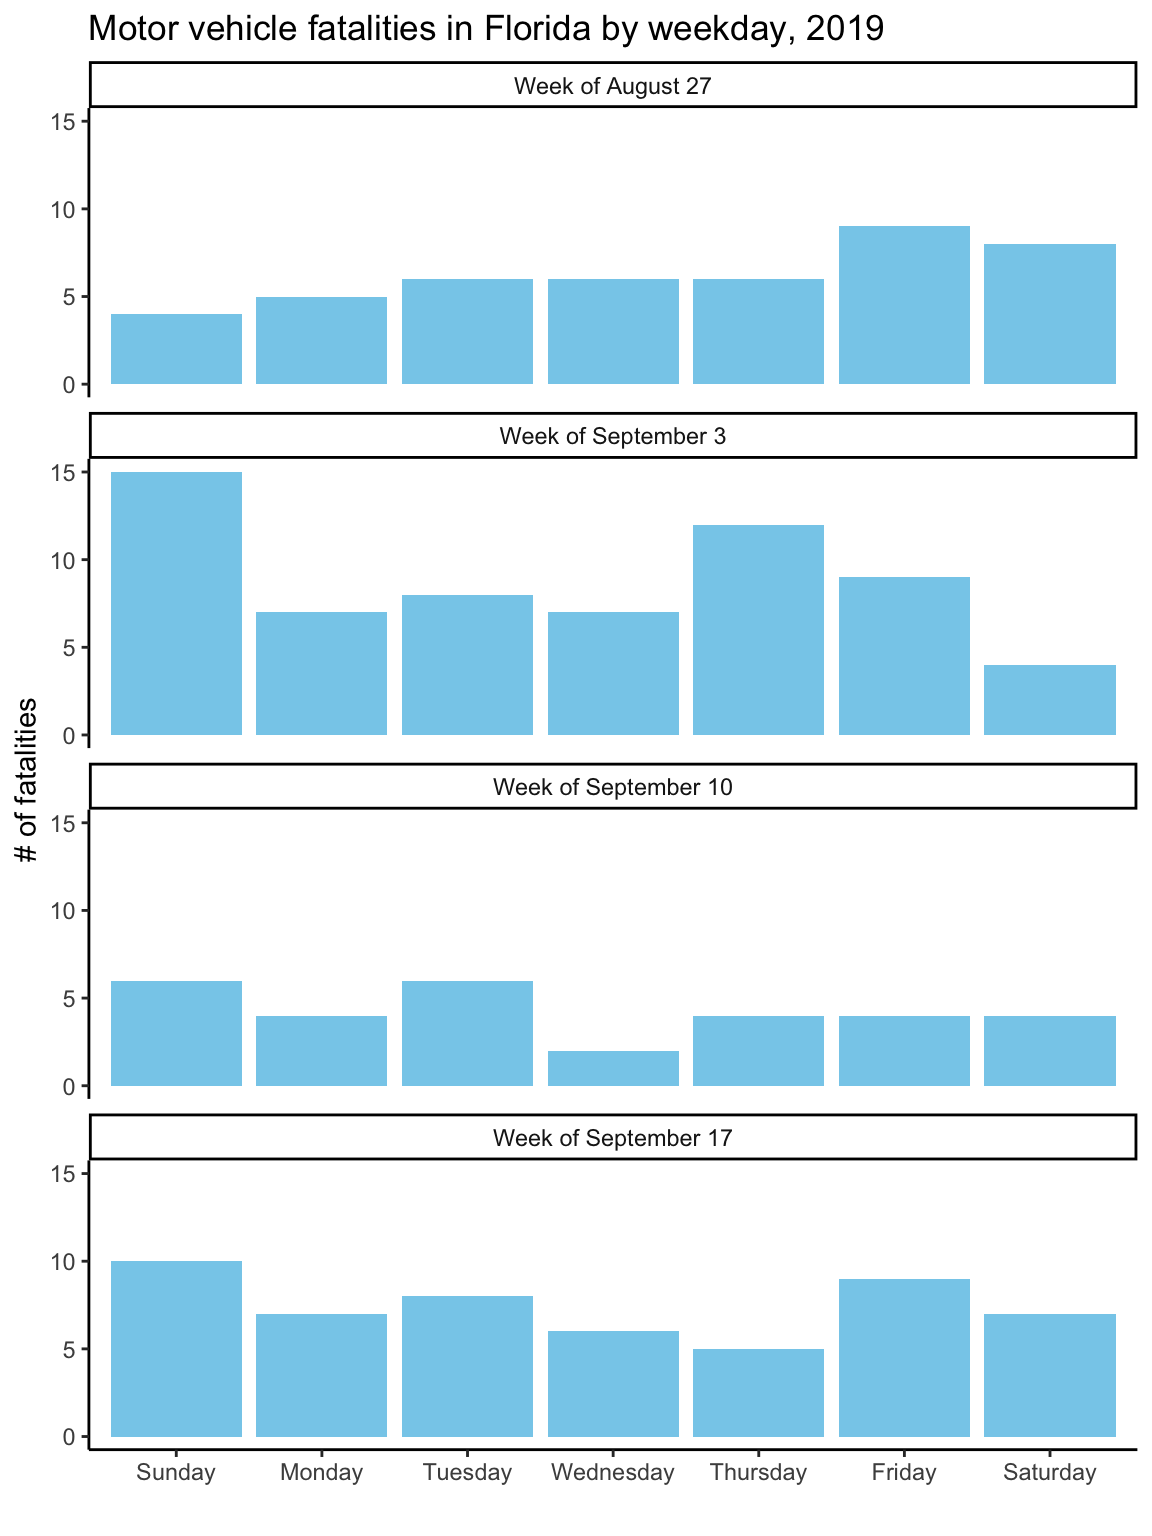
\includegraphics{navy_public_health_files/figure-latex/plotelements2-1} \caption[Number of motor vehicle fatalities in Florida by day of the week and week for the weeks surrounding Hurricane Irma's landfall]{Number of motor vehicle fatalities in Florida by day of the week and week for the weeks surrounding Hurricane Irma's landfall.}\label{fig:plotelements2}
\end{figure}

Here's the breakdown of plot elements for this plot:

\begin{itemize}
\tightlist
\item
  \textbf{data}: The data illustrated with this plot is the same as for Figure
  \ref{fig:plotelements2}, the example data
  shown in Table \ref{tab:exampledata}.
\item
  \textbf{geoms}: The geometric objects used to plot the data are columns.
\item
  \textbf{aesthetics}: For the column geoms, the x-axis position is mapped to the day
  of the week and the y-axis position is mapped to the number of fatalities. The
  color is mapped to a constant aesthetic, sky blue.
\item
  \textbf{coordinate system}: The plot uses a \textbf{Cartesian coordinate system}.
\item
  \textbf{scales}: The plot uses a default \textbf{discrete scale} for the x-axis and the
  default \textbf{continuous scale} for the y-axis.
\item
  \textbf{labels}: This plot uses the axis titles ``Date'' for the x-axis, ``\# of fatalities''
  for the y-axis, and ``Day of week'' for the color scale. In a minute, when you start
  working with the example data, you'll see that these are changed from the corresponding
  column names in the data, to make the plot easier to understand. In addition,
  the plot has both a title (``Motor vehicle fatalities in Florida'') and a
  subtitle (``Late summer / early fall of 2019'').
\item
  \textbf{theme}: This plot uses the \texttt{theme\_classic} theme, with a white background
  to the main plot area, no gridlines, a Sans Serif font family,
  and axis lines only on the left and bottom sides of the plot area.
\item
  \textbf{faceting}: This plot facets by week. This variable was obtained from the ``week''
  column in the dataset, although some changes were made to have better labeling of
  the facets (e.g., ``Week of August 27'' rather than ``35'').
\end{itemize}

\hypertarget{building-a-plot}{%
\section{Building a plot}\label{building-a-plot}}

\newthought{Now that you have} and idea of how different elements combine to
create a plot, I'll walk you through the steps to ``layer'' these elements together
to create these two example plots.

\hypertarget{reading-data}{%
\subsection{Reading data}\label{reading-data}}

First, you'll need to bring the example data into your R session. If you followed
the steps in the ``Prerequisites'' section, you should have a
\textbf{comma-separated file}\footnote{\textbf{comma-separated file format.} A flat file format
  (try opening the file in a plain text editor---unlike a binary file format like
  Excel, you should be able to read all the content) where each column entry is
  separated by a comma. This is a common file format for tabular data that can
  be read into and written from most statistical programs (including R, Excel, and
  SAS).} in a ``data'' subdirectory of your current working directory. Also, if you
followed the steps in the ``Prerequisites'' section, you should have installed
all the necessary R packages for this example.

While there are functions in base R that import comma-separated files, I think the
functions in the \textbf{readr} package \citep{R-readr}, a package in the \textbf{tidyverse},
has some nicer defaults. To use functions in this package, you first need to load
it into your R session using the \texttt{library} function:

\begin{Shaded}
\begin{Highlighting}[]
\KeywordTok{library}\NormalTok{(}\StringTok{"readr"}\NormalTok{)}
\end{Highlighting}
\end{Shaded}

The \texttt{library} function must specify the name of the package you'd like to load (in
this case, ``readr''). If you have forgotten to install the ``readr'' package before you
run this function, you'll get the message:

\begin{verbatim}
Error in library(readr) : there is no package called ‘readr’
\end{verbatim}

If you get that message, go back and re-read the ``Prerequisites'' to make sure you've
installed all the required packages.\footnote{There is also a small chance, especially if
  you're using a computer for which you don't have superuser privileges, that something
  else is going on. Double-check that you installed the package you're trying to load,
  and if loading the package still doesn't work, talk with your IT team about
  installing and loading R packages on your computer. For some company- or
  government-issued computers, the computer might have been set up to restrict
  installing new software, or to save installed software somewhere other than the
  default locations where R searches with \texttt{library}.}

Now that you've loaded \texttt{readr}, you can use the package's \texttt{read\_csv} function\footnote{For
  this and any other R function, you can open a help file in RStudio to give you
  more information about the function, usually including some examples of how to
  use if. Just type \texttt{?} and then the function name---for this example, \texttt{?read\_csv}.}
to read in the data. The one argument this function requires is the
\textbf{file path}\footnote{\textbf{file path.} The directions for where to find a file within your
  computer's directory structure. If the file you want is in your current working
  directory, this will just be the filename of the file. If it's not, but in a directory
  close-by, you can use a \emph{relative pathname} to give the directions from the current
  working directory. Since the file you want to read in is in a subdirectory called
  ``data'' of the current working directory, the filepath here is
  ``data/daily\_fatalities.csv''.}
to the data file.

\begin{Shaded}
\begin{Highlighting}[]
\NormalTok{daily_fatalities <-}\StringTok{ }\KeywordTok{read_csv}\NormalTok{(}\StringTok{"data/daily_fatalities.csv"}\NormalTok{)}
\end{Highlighting}
\end{Shaded}

\begin{verbatim}
## Parsed with column specification:
## cols(
##   date = col_date(format = ""),
##   week = col_double(),
##   weekday = col_character(),
##   fatals = col_double()
## )
\end{verbatim}

Don't be alarmed by the message that's printed out after you run the function!
In data frames in R, each columns can have one of several different classes
(some examples: character: ``Florida'', date: 2017-09-10, integer: 17,
double: 17.0). The \texttt{read\_csv} function looks at the values in each column in the
data and tries to guess what class each column should be, and this message
tells you what it guessed, so you can check. In this case, the number of
fatalities will always be a whole number, so the ``integer'' class would have
also worked well, but there should be no problem with the column having a
``double'' class for the plotting we'll be doing, so everything looks fine.

The previous code used a \textbf{gets arrow}\footnote{\textbf{gets arrow.} The function
  \texttt{\textless{}-}, which allows you to save the output from running the code on the right-hand
  side of the arrow to an object with the name on the left of the arrow. This is a
  funny kind of function called an \textbf{infix function}, which goes between two
  function arguments instead of putting the arguments inside parentheses. If you
  want to look up the helpfile for an infix function, wrap it in backticks:
  \texttt{?\textasciigrave{}\textless{}-\textasciigrave{}}.} to save the data you read in to an R object called \texttt{daily\_fatalities}.
Now, anytime you want to use this data, you can reference it with the name
\texttt{daily\_fatalities} instead of needing to read it in again. For example, you
can print out the start of the data by calling the object name by itself:

\begin{Shaded}
\begin{Highlighting}[]
\NormalTok{daily_fatalities}
\end{Highlighting}
\end{Shaded}

\begin{verbatim}
## # A tibble: 28 x 4
##    date        week weekday   fatals
##    <date>     <dbl> <chr>      <dbl>
##  1 2017-08-27    35 Sunday         4
##  2 2017-08-28    35 Monday         5
##  3 2017-08-29    35 Tuesday        6
##  4 2017-08-30    35 Wednesday      6
##  5 2017-08-31    35 Thursday       6
##  6 2017-09-01    35 Friday         9
##  7 2017-09-02    35 Saturday       8
##  8 2017-09-03    36 Sunday        15
##  9 2017-09-04    36 Monday         7
## 10 2017-09-05    36 Tuesday        8
## # ... with 18 more rows
\end{verbatim}

By default, \texttt{read\_csv} read the data into a structure called a \textbf{tibble},\footnote{\textbf{tibble.}
  A slightly fancier dataframe, which is a tabular data format in R, where there are
  rows and columns, with each column having data with the same class (e.g., character,
  integer, date) and all columns having the same length. Values in the columns should
  ``line up'' across the rows---for example, in this case, the second value in the
  \texttt{fatals} column should be the number of fatalities for the date given by the second
  value in the \texttt{date} column. Compared to a dataframe, a tibble prints out more nicely
  when you call the object name alone, among some other advantages.} and you
can see that the top of the print-out notes this. It also gives the dimensions
(28 rows and 4 columns) and, under each column name, the class of the column.
When you start plotting this data, you'll use the dataframe's object name
(\texttt{daily\_fatalities}) to reference the full dataset and each column name
(e.g., \texttt{date} for the date of the observations, \texttt{fatals} for the number of
fatalities observed on that date) to reference specific elements of the data.

\hypertarget{plotting-by-layers}{%
\subsection{Plotting by layers}\label{plotting-by-layers}}

To create a data visualization using \texttt{ggplot2}, we'll add up ``layers'' for each of
the plot elements described earlier. In this section, I'll step through this process.
First, we'll create a \textbf{ggplot object} using the \texttt{ggplot} call, and then we'll add
layers to it with \texttt{+}. To use these functions, you'll need to load the \texttt{ggplot2}
package:

\begin{Shaded}
\begin{Highlighting}[]
\KeywordTok{library}\NormalTok{(ggplot2)}
\end{Highlighting}
\end{Shaded}

For the first step, create the \texttt{ggplot} object. When you create this object, specify
the dataframe with the data you'd like to plot using the \texttt{data} parameter:

\begin{Shaded}
\begin{Highlighting}[]
\KeywordTok{ggplot}\NormalTok{(}\DataTypeTok{data =}\NormalTok{ daily_fatalities)}
\end{Highlighting}
\end{Shaded}

\begin{figure*}

\includegraphics{navy_public_health_files/figure-latex/step1-1} \caption[Step 1 of layering a plot]{Step 1 of layering a plot: Creating the ggplot object. At this point, nothing's actually plotted, because we haven't added any geoms yet.}\label{fig:step1}
\end{figure*}

Figure \ref{fig:step1} shows the output with this single, initial layer. We haven't added any geoms yet, so the plot isn't showing anything. Since we've specified the
data, however, we'll be able to add geoms where we map aesthetics to columns in the
dataset. Let's do that next, and add a layer with a line (\texttt{geom\_line}) for the number
of fatalities per day. We'll use the \texttt{aes} function \emph{inside} the \texttt{geom\_line} call
to specify that we want the x-axis to show the value in the \texttt{date} column and the
y-axis to show the value in the \texttt{fatals} column:

\begin{Shaded}
\begin{Highlighting}[]
\KeywordTok{ggplot}\NormalTok{(}\DataTypeTok{data =}\NormalTok{ daily_fatalities) }\OperatorTok{+}\StringTok{ }\KeywordTok{geom_line}\NormalTok{(}\KeywordTok{aes}\NormalTok{(}\DataTypeTok{x =}\NormalTok{ date, }
    \DataTypeTok{y =}\NormalTok{ fatals))}
\end{Highlighting}
\end{Shaded}

\begin{figure*}
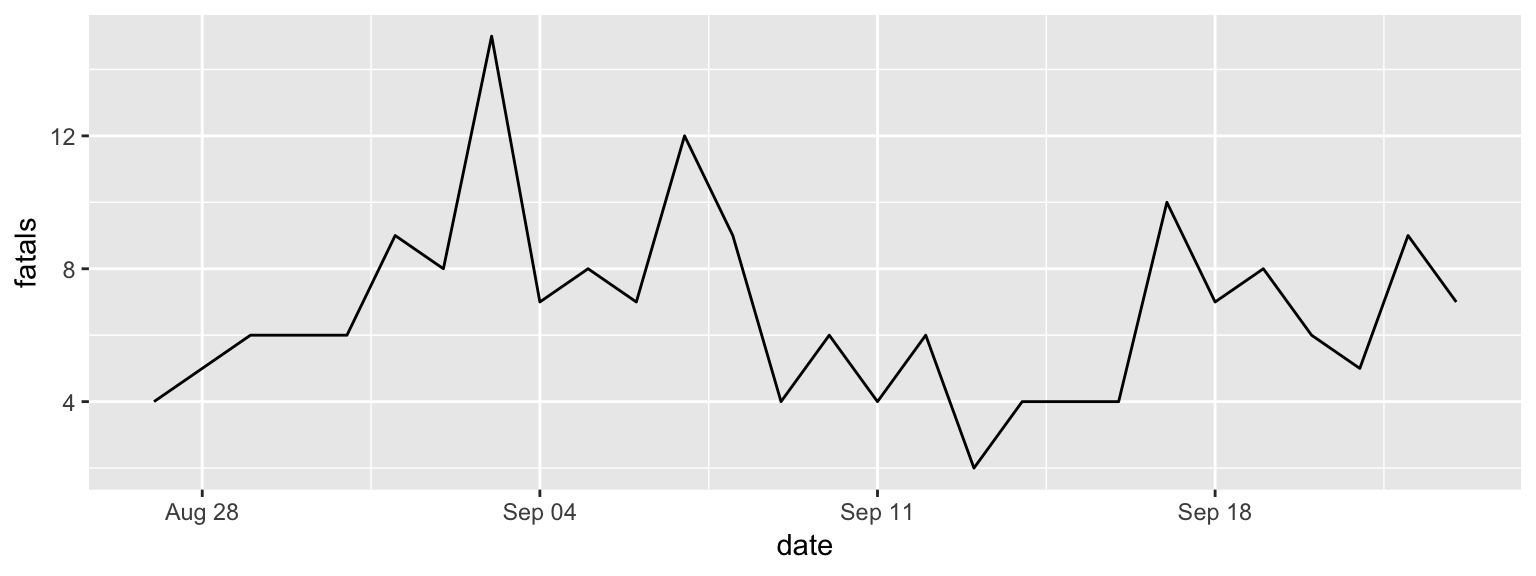
\includegraphics{navy_public_health_files/figure-latex/step2-1} \caption[Step 2 of layering a plot]{Step 2 of layering a plot: Adding a line geom. In this case, the x-axis (x aesthetic) is mapped to the 'date' column in the data, while the y-axis (y aesthetic) is mapped to the 'fatals' column.}\label{fig:step2}
\end{figure*}

The result is in Figure \ref{fig:step2}. You can see that you now have a line showing
the number of fatalities per day. Next, we can add a layer on top of the line with a
point (\texttt{geom\_point}) for each date showing the number of fatalities. Two of the
aesthetics for this geom (x and y) will be the same as for the line. However, we
also want to map color to day of the week. Since day of the week is in a column
called \texttt{weekday}, we can specify this aesthetic as \texttt{color\ =\ weekday} within the \texttt{aes}
call. Try running the following code to add this layer:

\begin{Shaded}
\begin{Highlighting}[]
\KeywordTok{ggplot}\NormalTok{(}\DataTypeTok{data =}\NormalTok{ daily_fatalities) }\OperatorTok{+}\StringTok{ }\KeywordTok{geom_line}\NormalTok{(}\KeywordTok{aes}\NormalTok{(}\DataTypeTok{x =}\NormalTok{ date, }
    \DataTypeTok{y =}\NormalTok{ fatals)) }\OperatorTok{+}\StringTok{ }\KeywordTok{geom_point}\NormalTok{(}\KeywordTok{aes}\NormalTok{(}\DataTypeTok{x =}\NormalTok{ date, }\DataTypeTok{y =}\NormalTok{ fatals, }
    \DataTypeTok{color =}\NormalTok{ weekday))}
\end{Highlighting}
\end{Shaded}

\begin{figure*}
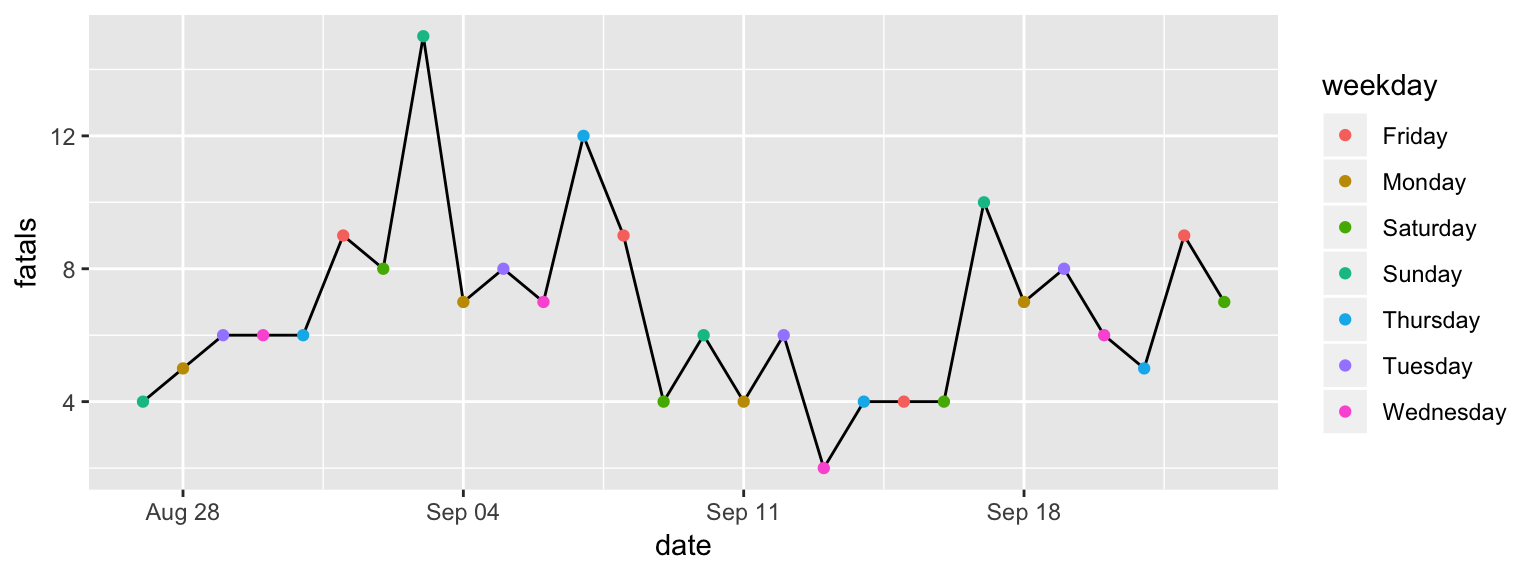
\includegraphics{navy_public_health_files/figure-latex/step3-1} \caption[Step 3 of layering a plot]{Step 3 of layering a plot: Adding a point geom. The x and y aesthetics are the same as for the line geom, but now we're also mapping color to the 'weekday' column in the data.}\label{fig:step3}
\end{figure*}

You should get the plot shown in Figure \ref{fig:step3}. You may have noticed that
the set of colors that is used for weekdays is different than in the plot in
Figure \ref{fig:plotelements}. This set of colors is actually specified by the
``scale'' element of the plot, so we'll change that in a different layer.

So far, we've customized some of the plot aesthetics by mapping them so that their
values are based on observations in the data. However, sometimes you'll want
to change an aesthetic to a \textbf{constant}, where the aesthetic changes for the
aesthetic for all of the observations from the data, but in the same way.

For example, for this plot, we'd like the line to be dark gray for all observations,
and we'd like the points to be a little bigger. To specify a \textbf{constant aesthetic},
move it outside of the \texttt{aes} call. For colors, you can set a constant value to
one of the many named ``R Colors''\footnote{See \href{http://www.stat.columbia.edu/~tzheng/files/Rcolor.pdf}{this website} for examples and names}
(make sure you put the color name inside parentheses---otherwise, R will think you're
refering to an R object). Constant point size values can be specified using numbers,
where larger numbers will make bigger points and the default value is somewhere
around 1.\footnote{For
  an in-depth look at aesthetic specifications, see
  \href{https://cran.r-project.org/web/packages/ggplot2/vignettes/ggplot2-specs.html}{the ggplot2 specs vignette}} Try numbers bigger than 1 (e.g., 1.5, 2) for bigger points and smaller
values (e.g., 0.8, 0.5) for smaller points.

The following code will set the line to be dark gray and the points to be a bit larger (result in Figure \ref{fig:step4}):

\begin{Shaded}
\begin{Highlighting}[]
\KeywordTok{ggplot}\NormalTok{(}\DataTypeTok{data =}\NormalTok{ daily_fatalities) }\OperatorTok{+}\StringTok{ }\KeywordTok{geom_line}\NormalTok{(}\KeywordTok{aes}\NormalTok{(}\DataTypeTok{x =}\NormalTok{ date, }
    \DataTypeTok{y =}\NormalTok{ fatals), }\DataTypeTok{color =} \StringTok{"darkgray"}\NormalTok{) }\OperatorTok{+}\StringTok{ }\KeywordTok{geom_point}\NormalTok{(}\KeywordTok{aes}\NormalTok{(}\DataTypeTok{x =}\NormalTok{ date, }
    \DataTypeTok{y =}\NormalTok{ fatals, }\DataTypeTok{color =}\NormalTok{ weekday), }\DataTypeTok{size =} \DecValTok{2}\NormalTok{)}
\end{Highlighting}
\end{Shaded}

\begin{figure*}
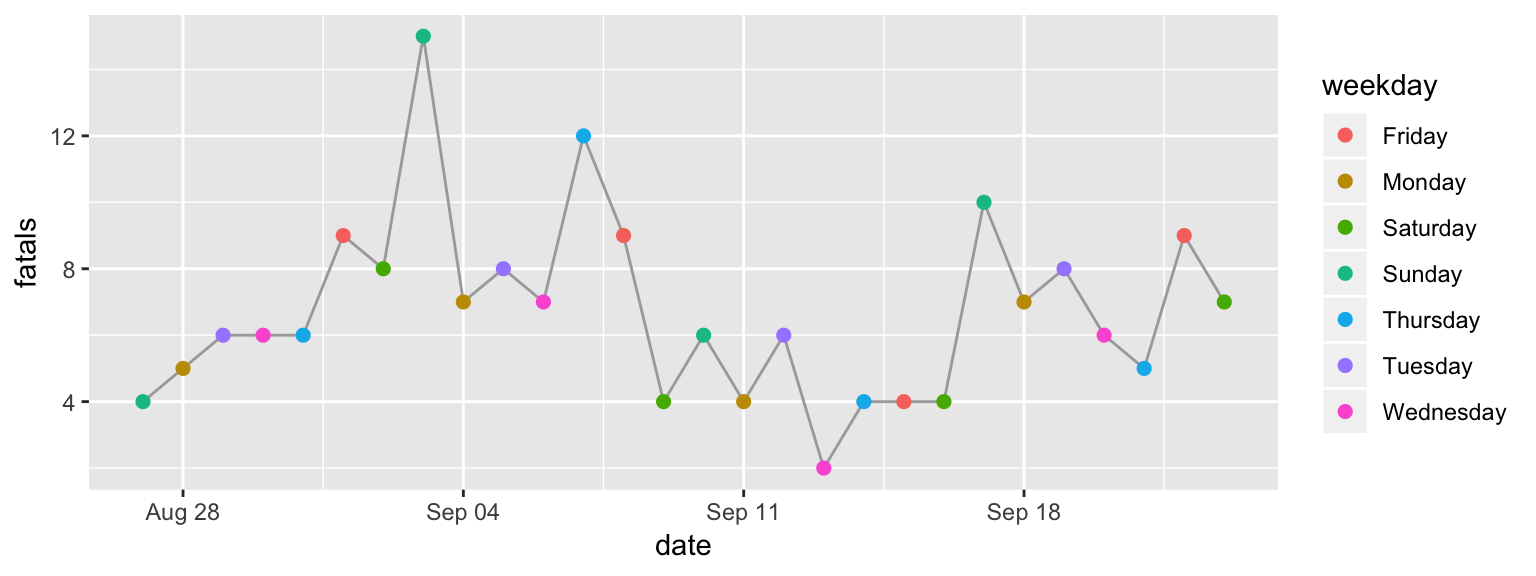
\includegraphics{navy_public_health_files/figure-latex/step4-1} \caption[Step 4 of layering a plot]{Step 4 of layering a plot: Adding constant aesthetics. In this step, we're making the line dark gray for all observations and the points a bit larger. Note that these aesthetics, since they're constant, are set outside of the 'aes' call. Also, note that thee color is specified inside quotation marks.}\label{fig:step4}
\end{figure*}

We're using the default coordinate system for this plot, so we don't need to add
a layer for the coordinate system. For plots where you need to change from this
default coordinate system, you'll add a layer that starts with \texttt{coord\_}. For example,
in the ``Map'' section, you'll see how to use a geographic coordinate system using
\texttt{coord\_map}. If you want to flip your x- and y-axis (there are a few examples where
this is useful), you can add a layer with \texttt{coord\_flip}.

While we're also using the default scales for the x aesthetic, we aren't for
the y or color aesthetic. The change to the y scale is very minimal: we're just
expanding it to include 0. This can be done by adding the layer \texttt{expand\_limits}
with the \texttt{y} parameter set to 0.

To change the color scale, you need to add a layer to specify
the alternative color scale. We'll use a color scale called
``viridis''. This is good for discrete data (like here, where we're showing day of
the week rather than a continuous number), it really shines when you're plotting
continuous values. The order of the scale is clear to those who are colorblind, and
it's also clear when printed out on a black-and-white printer.

To change the color scale to use this scale, add a layer with \texttt{scale\_color\_viridis\_d}.
The ``d'' here is for ``discrete''; if you were using color to show a continuous
value in the data (e.g., a column with an integer or double class), you'd
add a layer called \texttt{scale\_color\_viridis\_c} instead. The final result of these
scale customizations is shown in Figure \ref{fig:step5}.

\begin{Shaded}
\begin{Highlighting}[]
\KeywordTok{ggplot}\NormalTok{(}\DataTypeTok{data =}\NormalTok{ daily_fatalities) }\OperatorTok{+}\StringTok{ }\KeywordTok{geom_line}\NormalTok{(}\KeywordTok{aes}\NormalTok{(}\DataTypeTok{x =}\NormalTok{ date, }
    \DataTypeTok{y =}\NormalTok{ fatals), }\DataTypeTok{color =} \StringTok{"darkgray"}\NormalTok{) }\OperatorTok{+}\StringTok{ }\KeywordTok{geom_point}\NormalTok{(}\KeywordTok{aes}\NormalTok{(}\DataTypeTok{x =}\NormalTok{ date, }
    \DataTypeTok{y =}\NormalTok{ fatals, }\DataTypeTok{color =}\NormalTok{ weekday), }\DataTypeTok{size =} \DecValTok{2}\NormalTok{) }\OperatorTok{+}\StringTok{ }
\StringTok{    }\KeywordTok{expand_limits}\NormalTok{(}\DataTypeTok{y =} \DecValTok{0}\NormalTok{) }\OperatorTok{+}\StringTok{ }\KeywordTok{scale_color_viridis_d}\NormalTok{()}
\end{Highlighting}
\end{Shaded}

\begin{figure*}
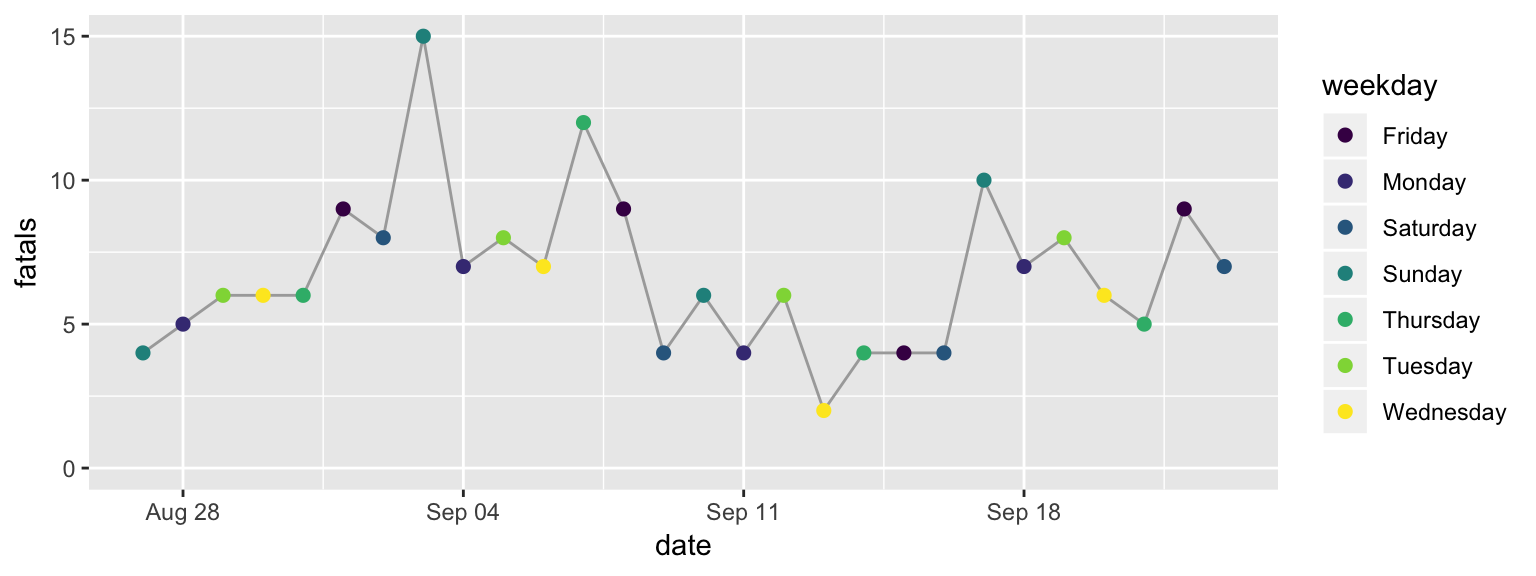
\includegraphics{navy_public_health_files/figure-latex/step5-1} \caption[Step 5 of layering a plot]{Step 5 of layering a plot: Changing the color scale. This step changes from the default color scale to the 'viridis' color scale.}\label{fig:step5}
\end{figure*}

The function for this layer has a few options for customization. For example, try
changing it to \texttt{scale\_color\_viridis\_d(option\ =\ "A")} or
\texttt{scale\_color\_viridis\_d(direction\ =\ -1)}. To see all its options, check its
helpfile with \texttt{?scale\_color\_viridis\_d}.

Next, we'll change the scale labels. By default, the label for each scale is the
name of the column in the data that the aesthetic was mapped to (x: ``date'',
y: ``fatals'', color: ``weekday''). You can add a \texttt{labs} layer to change these
to labels that are easier to understand. The other
labeling we'd like to do is to add a title and subtitle, which we can do with
a \texttt{ggtitle} layer (the subtitle is added with the \texttt{sub} parameter of this layer).
The final result of adding these layers is shown in Figure \ref{fig:step6}.

\begin{Shaded}
\begin{Highlighting}[]
\KeywordTok{ggplot}\NormalTok{(}\DataTypeTok{data =}\NormalTok{ daily_fatalities) }\OperatorTok{+}\StringTok{ }\KeywordTok{geom_line}\NormalTok{(}\KeywordTok{aes}\NormalTok{(}\DataTypeTok{x =}\NormalTok{ date, }
    \DataTypeTok{y =}\NormalTok{ fatals), }\DataTypeTok{color =} \StringTok{"darkgray"}\NormalTok{) }\OperatorTok{+}\StringTok{ }\KeywordTok{geom_point}\NormalTok{(}\KeywordTok{aes}\NormalTok{(}\DataTypeTok{x =}\NormalTok{ date, }
    \DataTypeTok{y =}\NormalTok{ fatals, }\DataTypeTok{color =}\NormalTok{ weekday), }\DataTypeTok{size =} \DecValTok{2}\NormalTok{) }\OperatorTok{+}\StringTok{ }
\StringTok{    }\KeywordTok{expand_limits}\NormalTok{(}\DataTypeTok{y =} \DecValTok{0}\NormalTok{) }\OperatorTok{+}\StringTok{ }\KeywordTok{scale_color_viridis_d}\NormalTok{() }\OperatorTok{+}\StringTok{ }
\StringTok{    }\KeywordTok{labs}\NormalTok{(}\DataTypeTok{x =} \StringTok{"Date"}\NormalTok{, }\DataTypeTok{y =} \StringTok{"# of fatalities"}\NormalTok{, }\DataTypeTok{color =} \StringTok{"Day of week"}\NormalTok{) }\OperatorTok{+}\StringTok{ }
\StringTok{    }\KeywordTok{ggtitle}\NormalTok{(}\StringTok{"Motor vehicle fatalities in Florida"}\NormalTok{, }
        \DataTypeTok{subtitle =} \StringTok{"Late summer / early fall of 2019"}\NormalTok{)}
\end{Highlighting}
\end{Shaded}

\begin{figure*}
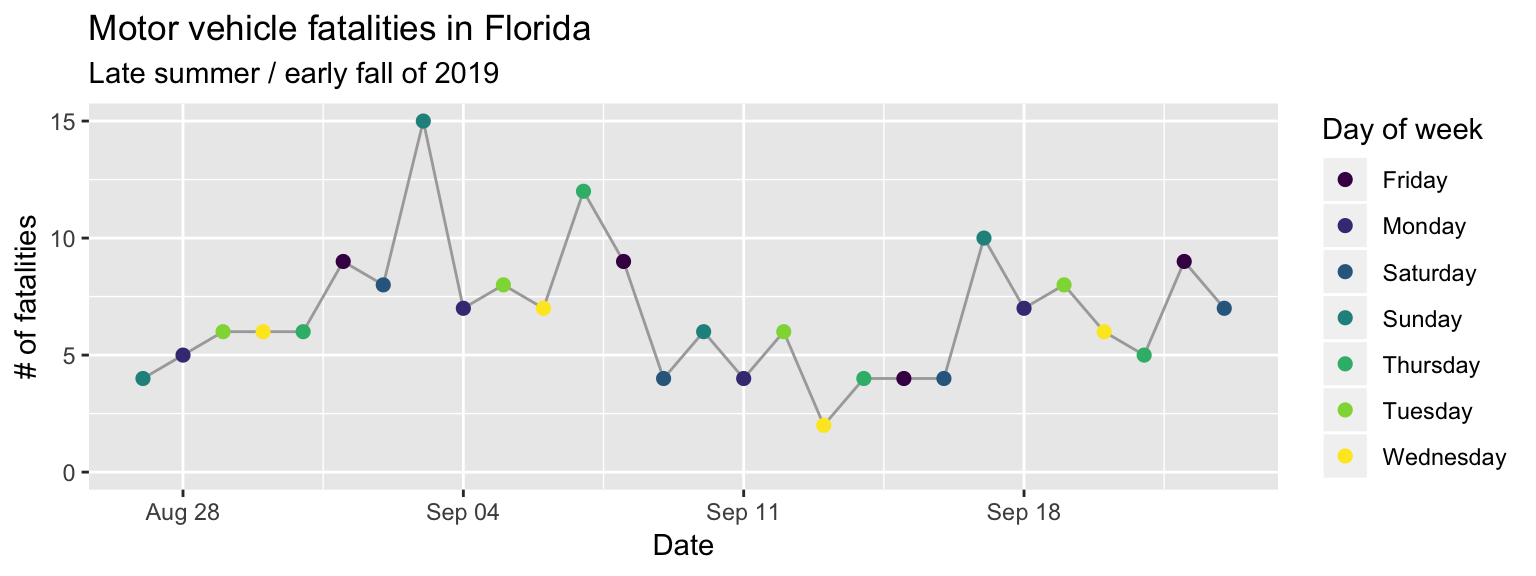
\includegraphics{navy_public_health_files/figure-latex/step6-1} \caption[Step 6 of layering a plot]{Step 6 of layering a plot: Customizing labels. The 'labs' layer customizes not only the x and y axis labels, but also the legend title for the color scale. The title and subtitle are added with a 'ggtitle' layer.}\label{fig:step6}
\end{figure*}

The last layer we need to add is a theme layer. While we're using most of the
elements from the default theme (\texttt{theme\_gray}), we do want to change the position
of the legend. For a time series plot like this, the change can be helpful, as it
lets us create a plot that's much wider than it is tall. You can move the legend
using the \texttt{theme} layer with an argument specified for \texttt{legend.position}. With
the \texttt{theme} function, you can customize almost any of the background elements of a
plot.\footnote{See the helpfile for ``theme'' with \texttt{?theme} for a full listing.}
However, you'll usually only want to do that for a few elements---if you want
to change a lot of elements, there is a set of functions that start \texttt{theme\_} that
will let you change to one of several ``themes'' that change many elements at once
(as I'll show in the next example).
If you find you're often using \texttt{theme} to specify lots of elements by hand, you
can create your own \texttt{theme\_*} function (fill in \texttt{*} with the name of your choice!).

\begin{Shaded}
\begin{Highlighting}[]
\KeywordTok{ggplot}\NormalTok{(}\DataTypeTok{data =}\NormalTok{ daily_fatalities) }\OperatorTok{+}\StringTok{ }\KeywordTok{geom_line}\NormalTok{(}\KeywordTok{aes}\NormalTok{(}\DataTypeTok{x =}\NormalTok{ date, }
    \DataTypeTok{y =}\NormalTok{ fatals), }\DataTypeTok{color =} \StringTok{"darkgray"}\NormalTok{) }\OperatorTok{+}\StringTok{ }\KeywordTok{geom_point}\NormalTok{(}\KeywordTok{aes}\NormalTok{(}\DataTypeTok{x =}\NormalTok{ date, }
    \DataTypeTok{y =}\NormalTok{ fatals, }\DataTypeTok{color =}\NormalTok{ weekday), }\DataTypeTok{size =} \DecValTok{2}\NormalTok{) }\OperatorTok{+}\StringTok{ }
\StringTok{    }\KeywordTok{expand_limits}\NormalTok{(}\DataTypeTok{y =} \DecValTok{0}\NormalTok{) }\OperatorTok{+}\StringTok{ }\KeywordTok{scale_color_viridis_d}\NormalTok{() }\OperatorTok{+}\StringTok{ }
\StringTok{    }\KeywordTok{labs}\NormalTok{(}\DataTypeTok{x =} \StringTok{"Date"}\NormalTok{, }\DataTypeTok{y =} \StringTok{"# of fatalities"}\NormalTok{, }\DataTypeTok{color =} \StringTok{"Day of week"}\NormalTok{) }\OperatorTok{+}\StringTok{ }
\StringTok{    }\KeywordTok{ggtitle}\NormalTok{(}\StringTok{"Motor vehicle fatalities in Florida"}\NormalTok{, }
        \DataTypeTok{subtitle =} \StringTok{"Late summer / early fall of 2019"}\NormalTok{) }\OperatorTok{+}\StringTok{ }
\StringTok{    }\KeywordTok{theme}\NormalTok{(}\DataTypeTok{legend.position =} \StringTok{"bottom"}\NormalTok{)}
\end{Highlighting}
\end{Shaded}

\begin{figure*}
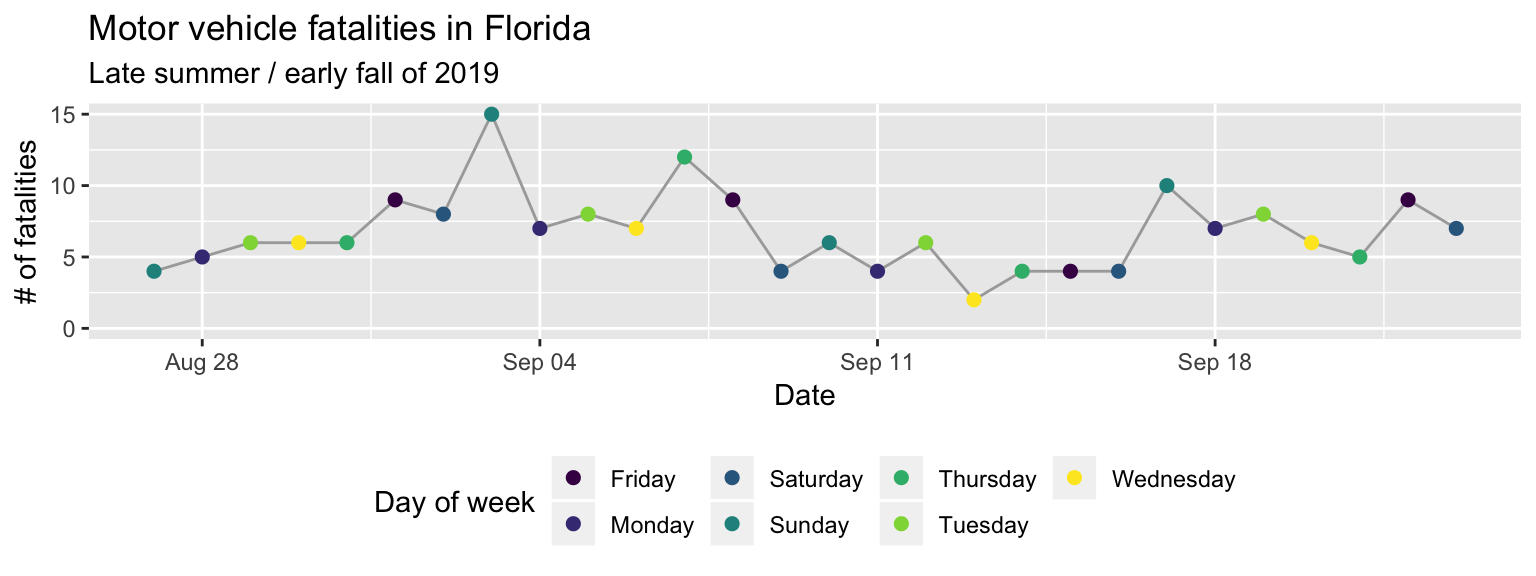
\includegraphics{navy_public_health_files/figure-latex/step7-1} \caption[Step 7 of layering a plot]{Step 7 of layering a plot: Customizing the theme. Move the color legend to below the plot.}\label{fig:step7}
\end{figure*}

As one final detail, if you were looking very closely, you may have noticed that
the order of the days of week are different in the original plot from our final
version here. That's because, by default, discrete character-class values are
ordered alphabetically. We can change this order, and should, to be the order that
week days occur. To do this, we need to change the column class to a
\textbf{factor class}\footnote{\textbf{factor class.} An R class for values that take character names,
  but that describe categories, for which you expect values to show up more than once
  in your data. In this data, the day of week is an example, since it is expressed
  as a character variable (``Monday'', ``Tuesday'', etc.), but we expect there to be
  multiple observations with, e.g., ``Monday''. If you have a varible that you expect
  to be unique (e.g., name of study subjects, unique ID number), the column should
  be in a character, not a factor, class.
  In R, each possible catogory for a factor is called a \textbf{level}.
  You can change the order of the levels of a factor, and this will change the
  order they're shown on a plot.} and then change the order of that factor's levels.

To do this, we'll need to load a few additional R packages (you'll also use these
in the ``Tidy'' section, which has much more on manipulating datasets). The
\textbf{forcats} package \citep{R-forcats} has functions for working with factors, including
a function we can use to reorder the factor levels. The \textbf{magrittr} package
\citep{R-magrittr} includes two infix functions we'll use to make the code
cleaner: the pipe operator (\texttt{\%\textgreater{}\%}) and the compound assignment pipe operator (\texttt{\%\textless{}\textgreater{}\%}).
The \textbf{dplyr} package \citep{R-dplyr} includes a number of simple but powerful functions
for manipulating tibbles.

The ``Tidy'' section will go into detail for how to use all these functions. As a brief
summary, the \texttt{mutate} function used twice to change the values in the ``weekday'' column:
first, to convert the class of the column to a factor (\texttt{as\_factor}) and second to
change the order of those levels (\texttt{fct\_relevel}) by hand, to start with Monday and
go in order through Sunday. The compound assignment pipe operator (\texttt{\%\textless{}\textgreater{}\%}) allows
us to perform all those operations to columns inside the ``daily\_fatalities'' tibble,
and then to save the result \emph{back to the same R object} (overwriting the earlier
version of the tibble).

\begin{Shaded}
\begin{Highlighting}[]
\KeywordTok{library}\NormalTok{(}\StringTok{"forcats"}\NormalTok{)}
\KeywordTok{library}\NormalTok{(}\StringTok{"magrittr"}\NormalTok{)}
\KeywordTok{library}\NormalTok{(}\StringTok{"dplyr"}\NormalTok{)}

\NormalTok{daily_fatalities }\OperatorTok\StringTok{ }\KeywordTok{mutate}\NormalTok{(}\DataTypeTok{weekday =} \KeywordTok{as_factor}\NormalTok{(weekday)) }\OperatorTok\StringTok{ }
\StringTok{    }\KeywordTok{mutate}\NormalTok{(}\DataTypeTok{weekday =} \KeywordTok{fct_relevel}\NormalTok{(weekday, }\StringTok{"Sunday"}\NormalTok{, }
        \StringTok{"Monday"}\NormalTok{, }\StringTok{"Tuesday"}\NormalTok{, }\StringTok{"Wednesday"}\NormalTok{, }\StringTok{"Thursday"}\NormalTok{, }
        \StringTok{"Friday"}\NormalTok{, }\StringTok{"Saturday"}\NormalTok{))}
\end{Highlighting}
\end{Shaded}

Now when we run the same \texttt{ggplot} code, you can see that the order of the days of
week in the color legend, and the order the colors are assigned to week day, have
changed (Figure \ref{fig:step8}).

\begin{Shaded}
\begin{Highlighting}[]
\KeywordTok{ggplot}\NormalTok{(}\DataTypeTok{data =}\NormalTok{ daily_fatalities) }\OperatorTok{+}\StringTok{ }\KeywordTok{geom_line}\NormalTok{(}\KeywordTok{aes}\NormalTok{(}\DataTypeTok{x =}\NormalTok{ date, }
    \DataTypeTok{y =}\NormalTok{ fatals), }\DataTypeTok{color =} \StringTok{"darkgray"}\NormalTok{) }\OperatorTok{+}\StringTok{ }\KeywordTok{geom_point}\NormalTok{(}\KeywordTok{aes}\NormalTok{(}\DataTypeTok{x =}\NormalTok{ date, }
    \DataTypeTok{y =}\NormalTok{ fatals, }\DataTypeTok{color =}\NormalTok{ weekday), }\DataTypeTok{size =} \DecValTok{2}\NormalTok{) }\OperatorTok{+}\StringTok{ }
\StringTok{    }\KeywordTok{expand_limits}\NormalTok{(}\DataTypeTok{y =} \DecValTok{0}\NormalTok{) }\OperatorTok{+}\StringTok{ }\KeywordTok{scale_color_viridis_d}\NormalTok{() }\OperatorTok{+}\StringTok{ }
\StringTok{    }\KeywordTok{labs}\NormalTok{(}\DataTypeTok{x =} \StringTok{"Date"}\NormalTok{, }\DataTypeTok{y =} \StringTok{"# of fatalities"}\NormalTok{, }\DataTypeTok{color =} \StringTok{"Day of week"}\NormalTok{) }\OperatorTok{+}\StringTok{ }
\StringTok{    }\KeywordTok{ggtitle}\NormalTok{(}\StringTok{"Motor vehicle fatalities in Florida"}\NormalTok{, }
        \DataTypeTok{subtitle =} \StringTok{"Late summer / early fall of 2019"}\NormalTok{) }\OperatorTok{+}\StringTok{ }
\StringTok{    }\KeywordTok{theme}\NormalTok{(}\DataTypeTok{legend.position =} \StringTok{"bottom"}\NormalTok{)}
\end{Highlighting}
\end{Shaded}

\begin{figure*}
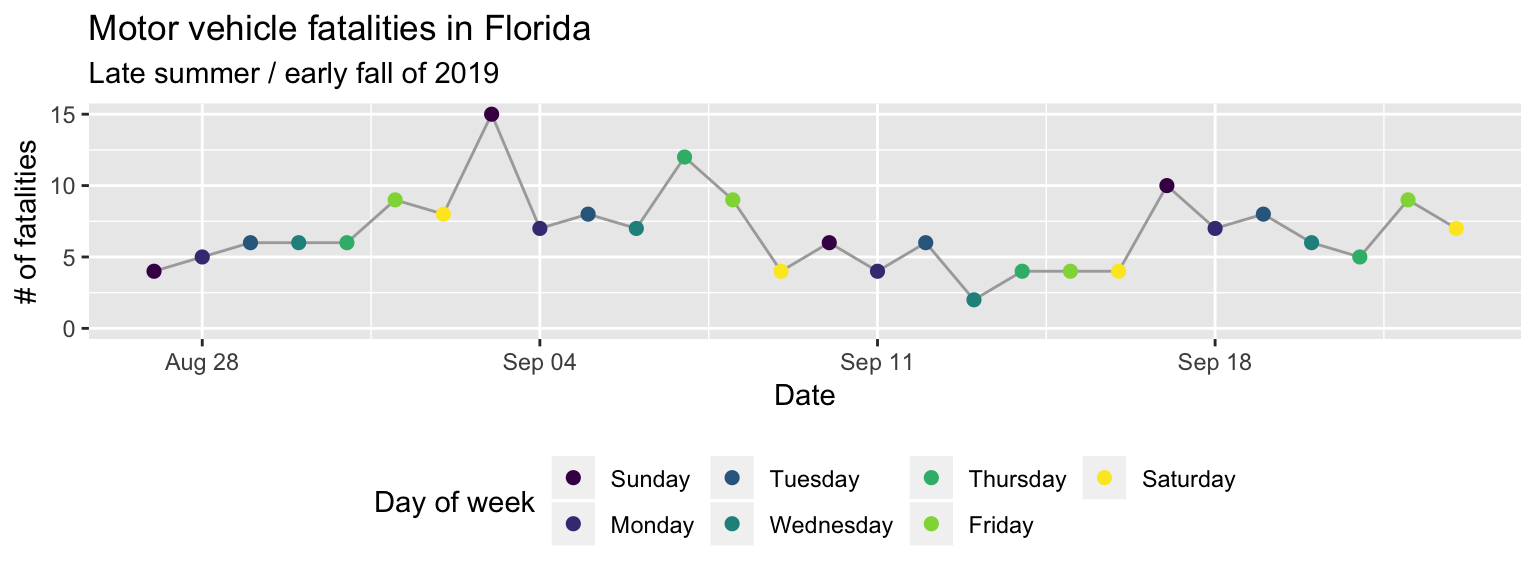
\includegraphics{navy_public_health_files/figure-latex/step8-1} \caption[Change the order of the days of week from alphabetical to temporal by transforming the data before plotting]{Change the order of the days of week from alphabetical to temporal by transforming the data before plotting.}\label{fig:step8}
\end{figure*}

The second example plot we can go through much more quickly. There are two
elements I'd like to point out: the layer for faceting and the layer for the theme.
The \texttt{facet\_wrap} function separates the plot into \textbf{small multiples}
based on the values in a column of the data. By default, all the scales (e.g., x-axis,
y-axis) will be the same across all the small multiples, allowing for an easier
comparison across the plots. The other layers in this code should now be somewhat
familiar to you: the \texttt{ggplot} call initializes a \texttt{ggplot} object with the
``daily\_fatalities'' dataset, just like in the last plot, while the \texttt{geom\_col} layer
adds a column geom where the x aesthetic is mapped to the value in the ``weekday''
column and the y aesthetic is mapped to the value in the ``fatals'' column.

\begin{figure}
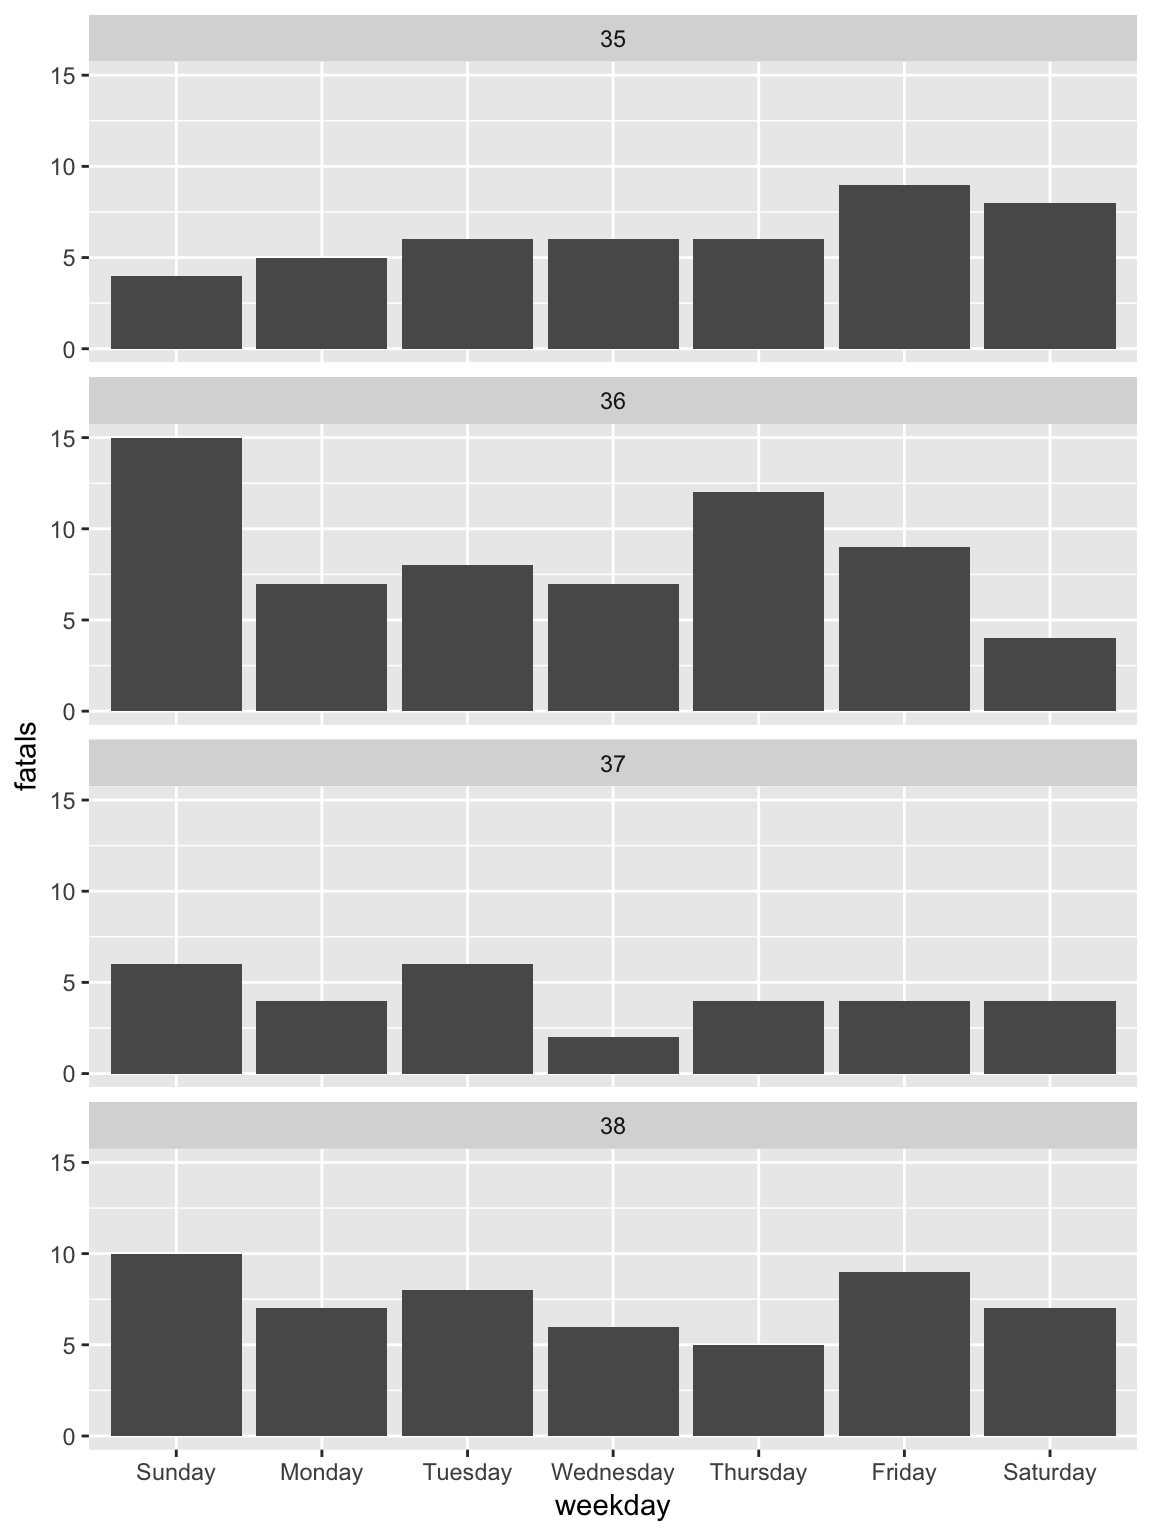
\includegraphics{navy_public_health_files/figure-latex/step1a-1} \caption[Adding a facet layer to a plot]{Adding a facet layer to a plot. The plot is now faceted by the 'week' column in the dataframe, with all the facets lined up vertically in a single column ('ncol = 1').}\label{fig:step1a}
\end{figure}

To change to the \texttt{theme\_classic}, all you need to do is add a \texttt{theme\_classic} layer
(Figure \ref{fig:step2a}).

\textbackslash{}begin\{figure\}
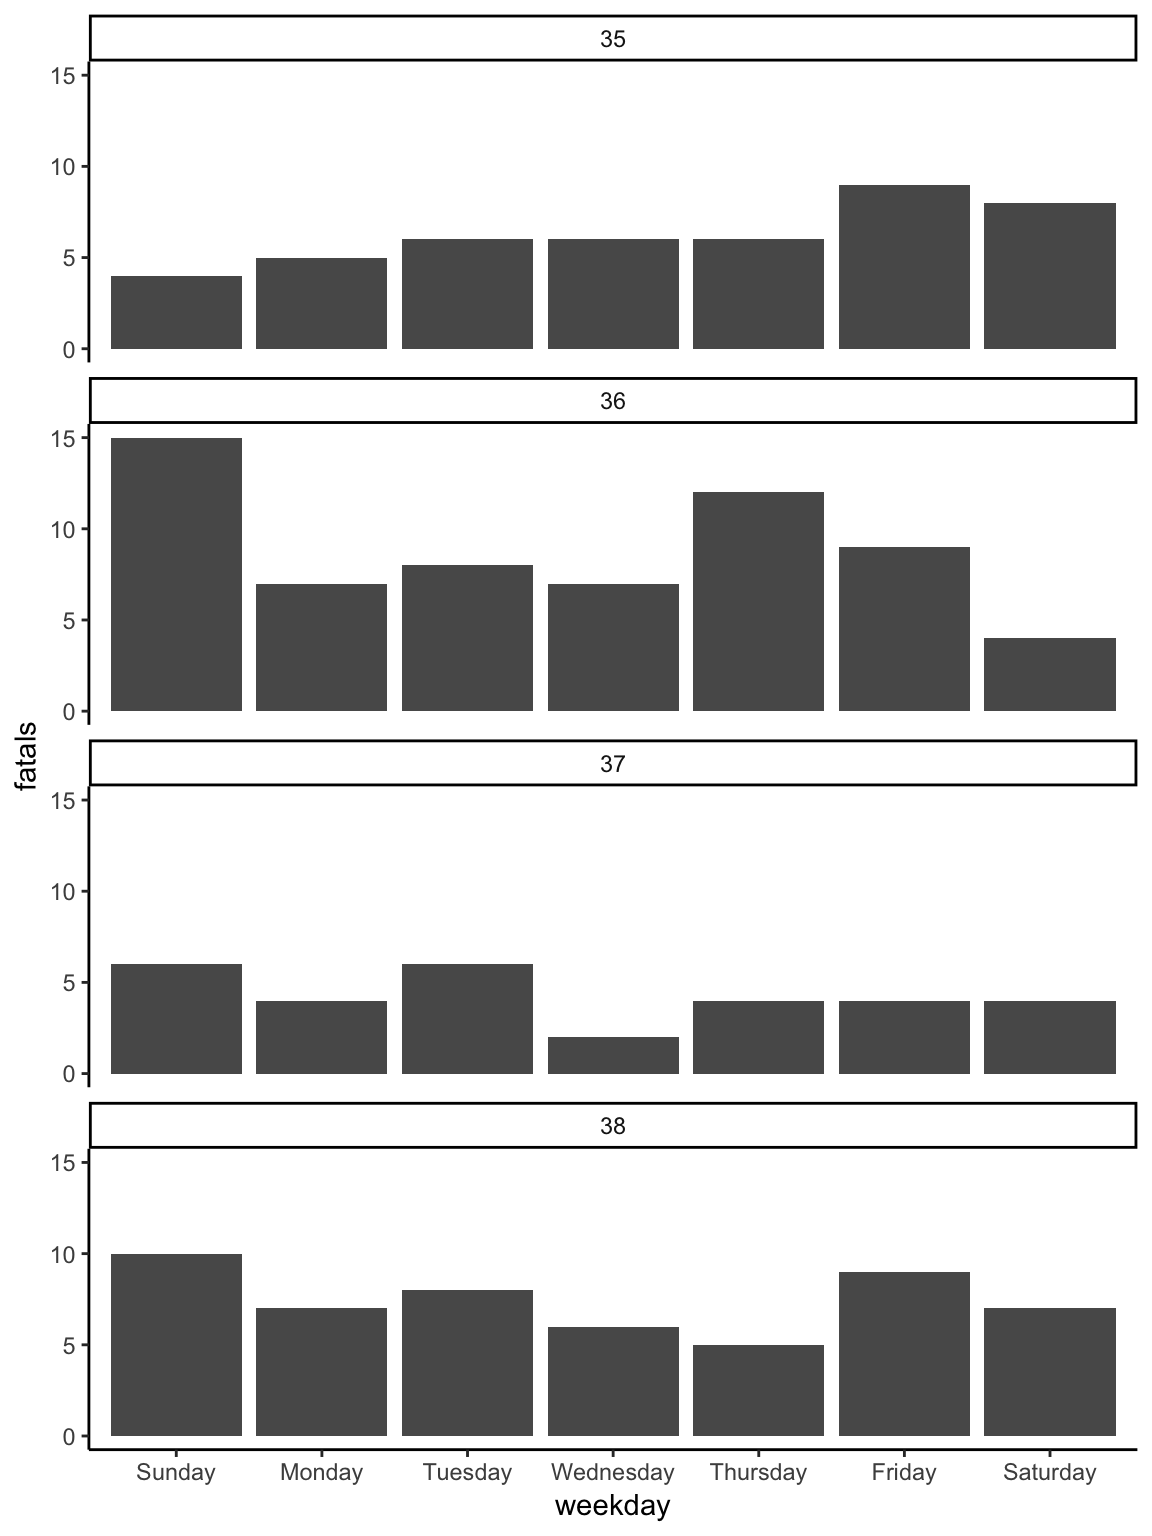
\includegraphics{navy_public_health_files/figure-latex/step2a-1} \textbackslash{}caption{[}Changing the theme{]}\{Changing the theme. The 'theme\_*' family of functions can quickly change many of the background elements of a plot with a single layer call.\}\label{fig:step2a}
\textbackslash{}end\{figure\}

Most of the rest of the layers for the plot are very similar to the first plot.
They include changing the \textbf{fill}\footnote{\textbf{fill aesthetic.} While all geoms have
  a \textbf{color aesthetic}, some also have a \textbf{fill} aesthetic. These include columns,
  bars, polygons, and points with certain shapes. In these cases, `color' will specify
  the outline of the geom while `fill' will specify the inside. Each geom has a set of
  required aesthetics and a set of possible aesthetics. To find each set for a geom,
  go to its helpfile (e.g., \texttt{?geom\_col}) and scroll down to the ``Aesthetics'' section.}
of the geom by mapping it to a constant fill
aesthetic (\texttt{color\ =\ "skyblue"} in the \texttt{geom\_col} call), customizing the labels with
a \texttt{lab} layer, and adding a title with \texttt{ggtitle}. The result of adding these layers
is shown in Figure \ref{fig:step3a}

\begin{Shaded}
\begin{Highlighting}[]
\KeywordTok{ggplot}\NormalTok{(}\DataTypeTok{data =}\NormalTok{ daily_fatalities) }\OperatorTok{+}\StringTok{ }\KeywordTok{geom_col}\NormalTok{(}\KeywordTok{aes}\NormalTok{(}\DataTypeTok{x =}\NormalTok{ weekday, }
    \DataTypeTok{y =}\NormalTok{ fatals), }\DataTypeTok{fill =} \StringTok{"skyblue"}\NormalTok{) }\OperatorTok{+}\StringTok{ }\KeywordTok{facet_wrap}\NormalTok{(}\OperatorTok{~}\NormalTok{week, }
    \DataTypeTok{ncol =} \DecValTok{1}\NormalTok{) }\OperatorTok{+}\StringTok{ }\KeywordTok{theme_classic}\NormalTok{() }\OperatorTok{+}\StringTok{ }\KeywordTok{labs}\NormalTok{(}\DataTypeTok{x =} \StringTok{""}\NormalTok{, }
    \DataTypeTok{y =} \StringTok{"# of fatalities"}\NormalTok{) }\OperatorTok{+}\StringTok{ }\KeywordTok{ggtitle}\NormalTok{(}\StringTok{"Motor vehicle fatalities in Florida by weekday, 2019"}\NormalTok{)}
\end{Highlighting}
\end{Shaded}

\begin{figure}
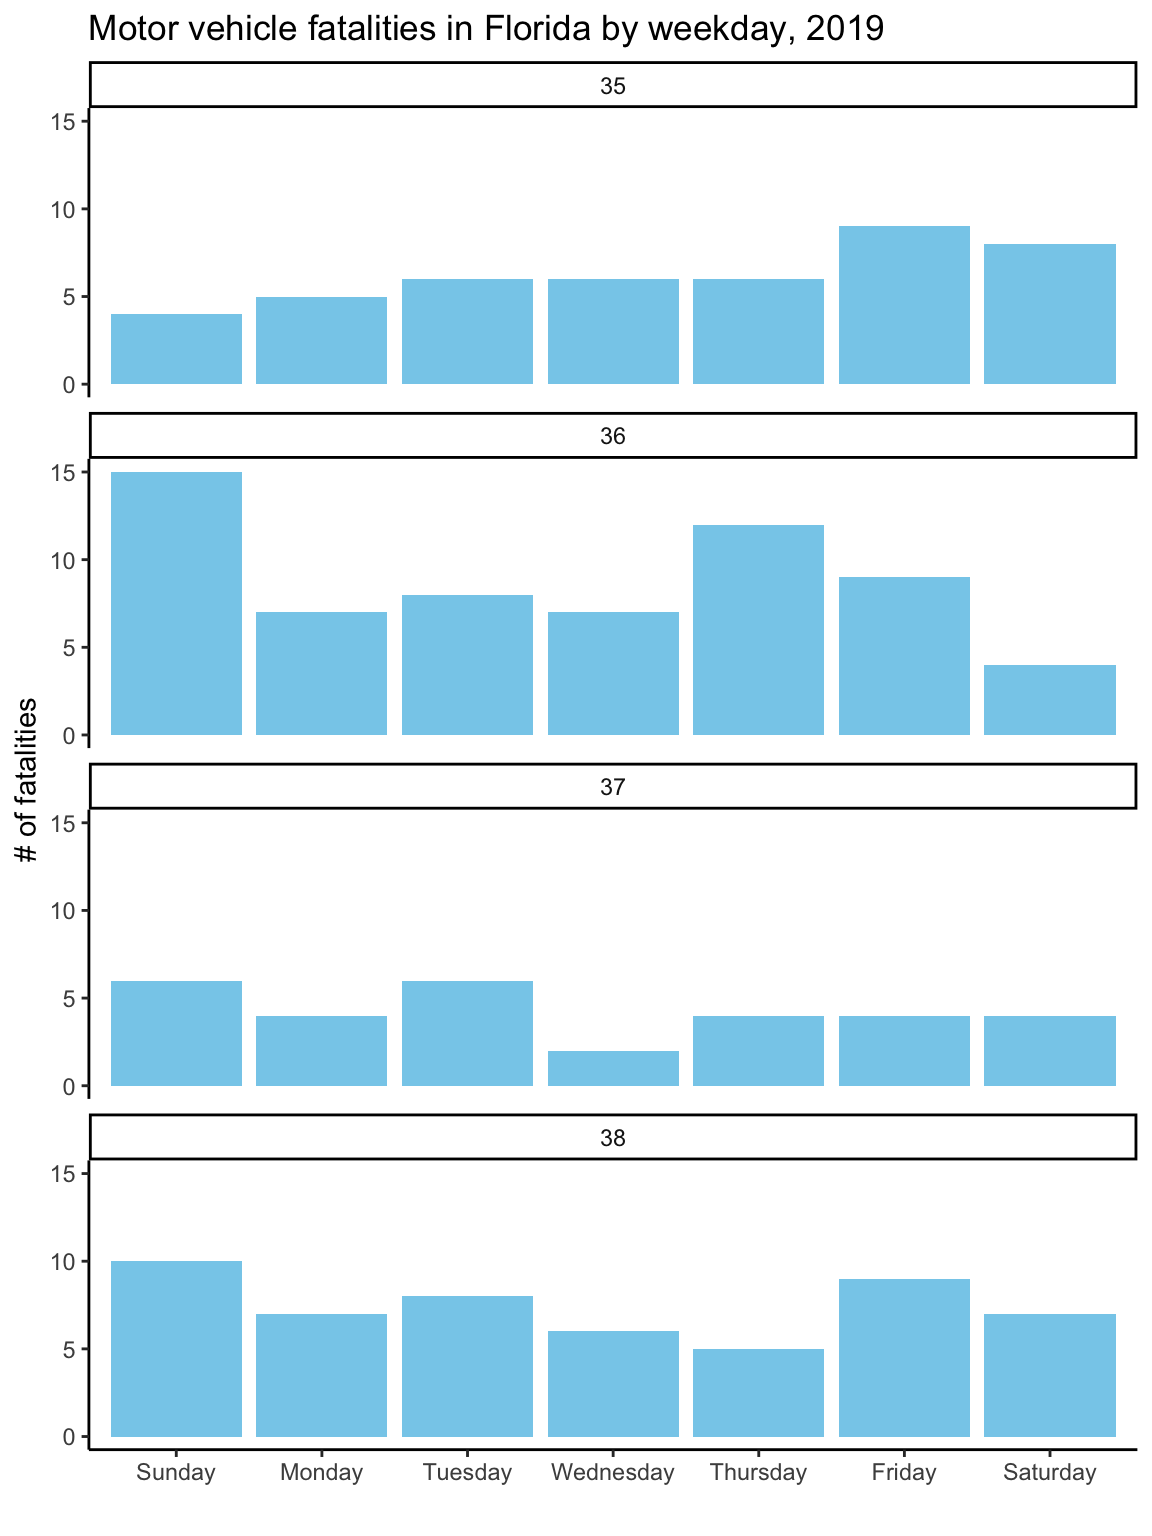
\includegraphics{navy_public_health_files/figure-latex/step3a-1} \caption[Customizing the labeling and adding a constant fill aesthetic]{Customizing the labeling and adding a constant fill aesthetic. Note that the constant fill aesthetic is specified outside the 'aes' call for the geom, and that the color is specified inside quotation marks.}\label{fig:step3a}
\end{figure}

As with the first graph, to take the plot to its final stage, you'll need to
change the input data a bit. In this case, this step is to create clearer labels for
the facets. The week number (e.g., 35) won't mean much to most viewers. A label giving
the date of the first day in the week (``Week of August 27'') will be more helpful.
To create these new labels, you can use \texttt{group\_by}, \texttt{mutate}, and \texttt{first} functions
from the \texttt{dplyr} package (which you have already loaded if you've worked through
the examples in order) to create a column called `first\_day' with the date of the
first day in each week. Then you can use \texttt{mutate} (also from \texttt{dplyr}) to create the
`week\_label' column from the existing columns of the tibble. This code uses the
\texttt{month} and \texttt{day} functions from the \texttt{lubridate} package (very useful for
working with dates) \citep{R-lubridate} to extract the month and day from the `first\_day'
dates, and then \texttt{paste} (from base R) pastes these together with ``Week of''.
Finally, the \texttt{as\_factor} and \texttt{fct\_reorder} calls (both from \texttt{forcats}, which you
also should have loaded if you've followed the examples in order) get this new
column in the right order, so that the facets show up in temporal order rather
than alphabetical.

Once you've made these changes to the `daily\_fatalities' tibble, you should get the
final version of the plot when you re-run the plotting code used in the last step,
getting Figure \ref{fig:step4a}.

\begin{Shaded}
\begin{Highlighting}[]
\KeywordTok{library}\NormalTok{(lubridate)}

\NormalTok{daily_fatalities }\OperatorTok\StringTok{ }\KeywordTok{group_by}\NormalTok{(week) }\OperatorTok\StringTok{ }\KeywordTok{mutate}\NormalTok{(}\DataTypeTok{first_day =} \KeywordTok{first}\NormalTok{(date)) }\OperatorTok\StringTok{ }
\StringTok{    }\KeywordTok{ungroup}\NormalTok{() }\OperatorTok\StringTok{ }\KeywordTok{mutate}\NormalTok{(}\DataTypeTok{week_label =} \KeywordTok{paste}\NormalTok{(}\StringTok{"Week of"}\NormalTok{, }
    \KeywordTok{month}\NormalTok{(first_day, }\DataTypeTok{label =} \OtherTok{TRUE}\NormalTok{, }\DataTypeTok{abbr =} \OtherTok{FALSE}\NormalTok{), }
    \KeywordTok{day}\NormalTok{(first_day))) }\OperatorTok\StringTok{ }\KeywordTok{mutate}\NormalTok{(}\DataTypeTok{week_label =} \KeywordTok{as_factor}\NormalTok{(week_label), }
    \DataTypeTok{week_label =} \KeywordTok{fct_reorder}\NormalTok{(week_label, week, }
        \DataTypeTok{.fun =}\NormalTok{ min))}

\KeywordTok{ggplot}\NormalTok{(}\DataTypeTok{data =}\NormalTok{ daily_fatalities) }\OperatorTok{+}\StringTok{ }\KeywordTok{geom_col}\NormalTok{(}\KeywordTok{aes}\NormalTok{(}\DataTypeTok{x =}\NormalTok{ weekday, }
    \DataTypeTok{y =}\NormalTok{ fatals), }\DataTypeTok{fill =} \StringTok{"skyblue"}\NormalTok{) }\OperatorTok{+}\StringTok{ }\KeywordTok{facet_wrap}\NormalTok{(}\OperatorTok{~}\NormalTok{week_label, }
    \DataTypeTok{ncol =} \DecValTok{1}\NormalTok{) }\OperatorTok{+}\StringTok{ }\KeywordTok{labs}\NormalTok{(}\DataTypeTok{x =} \StringTok{""}\NormalTok{, }\DataTypeTok{y =} \StringTok{"# of fatalities"}\NormalTok{) }\OperatorTok{+}\StringTok{ }
\StringTok{    }\KeywordTok{theme_classic}\NormalTok{() }\OperatorTok{+}\StringTok{ }\KeywordTok{ggtitle}\NormalTok{(}\StringTok{"Motor vehicle fatalities in Florida by weekday, 2019"}\NormalTok{)}
\end{Highlighting}
\end{Shaded}

\textbackslash{}begin\{figure\}
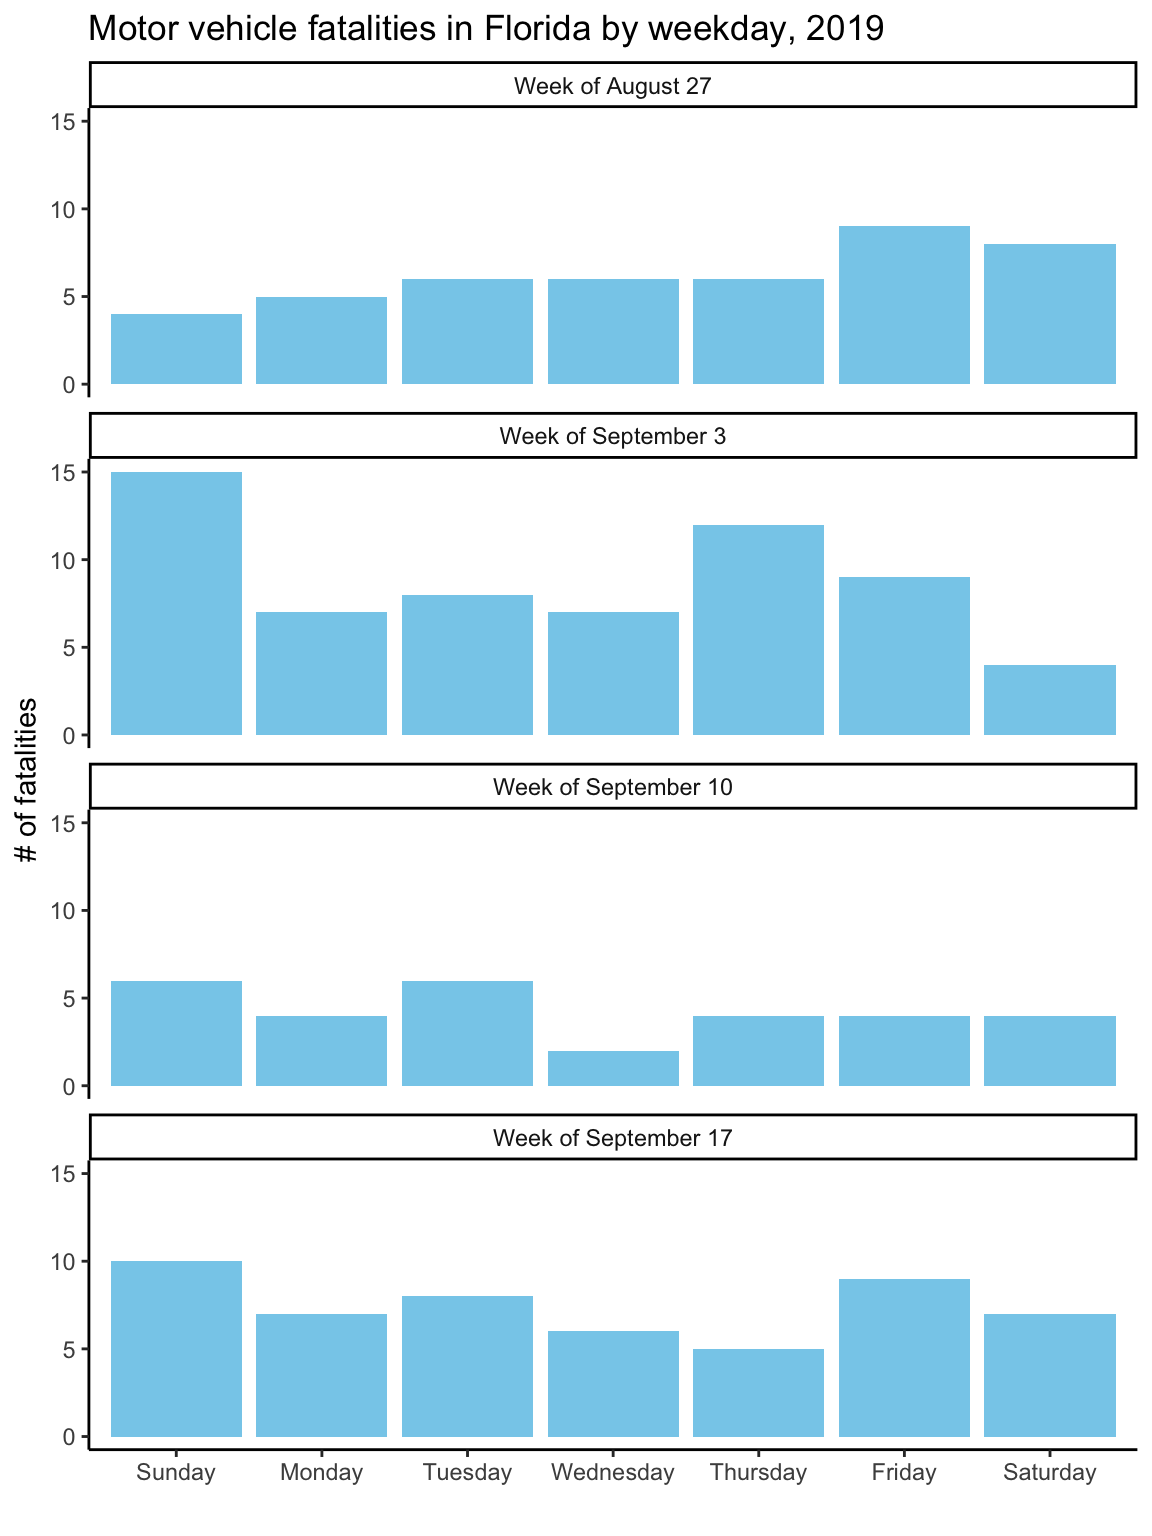
\includegraphics{navy_public_health_files/figure-latex/step4a-1} \textbackslash{}caption{[}To create better facet labels, you can first make some changes to the dataset and then facet by the newly created `week\_label' column rather than the `week' column{]}\{To create better facet labels, you can first make some changes to the dataset and then facet by the newly created `week\_label' column rather than the `week' column.\}\label{fig:step4a}
\textbackslash{}end\{figure\}

\hypertarget{saving-plots}{%
\section{Saving plots}\label{saving-plots}}

You can assign the output of a \texttt{ggplot} call to an R object using the gets arrow
(\texttt{\textless{}-}), just like you can assign data you've read in to an R object. If you do this,
the plot won't print immediately after you run the code:

\begin{Shaded}
\begin{Highlighting}[]
\NormalTok{irma_fatalities_plot <-}\StringTok{ }\KeywordTok{ggplot}\NormalTok{(}\DataTypeTok{data =}\NormalTok{ daily_fatalities) }\OperatorTok{+}\StringTok{ }
\StringTok{    }\KeywordTok{geom_col}\NormalTok{(}\KeywordTok{aes}\NormalTok{(}\DataTypeTok{x =}\NormalTok{ weekday, }\DataTypeTok{y =}\NormalTok{ fatals), }\DataTypeTok{fill =} \StringTok{"skyblue"}\NormalTok{) }\OperatorTok{+}\StringTok{ }
\StringTok{    }\KeywordTok{facet_wrap}\NormalTok{(}\OperatorTok{~}\NormalTok{week_label, }\DataTypeTok{ncol =} \DecValTok{1}\NormalTok{) }\OperatorTok{+}\StringTok{ }\KeywordTok{labs}\NormalTok{(}\DataTypeTok{x =} \StringTok{""}\NormalTok{, }
    \DataTypeTok{y =} \StringTok{"# of fatalities"}\NormalTok{) }\OperatorTok{+}\StringTok{ }\KeywordTok{theme_classic}\NormalTok{() }\OperatorTok{+}\StringTok{ }
\StringTok{    }\KeywordTok{ggtitle}\NormalTok{(}\StringTok{"Motor vehicle fatalities in Florida by weekday, 2019"}\NormalTok{)}
\end{Highlighting}
\end{Shaded}

However, now you can print the plot anytime you want by calling the object:

\begin{Shaded}
\begin{Highlighting}[]
\NormalTok{irma_fatalities_plot}
\end{Highlighting}
\end{Shaded}

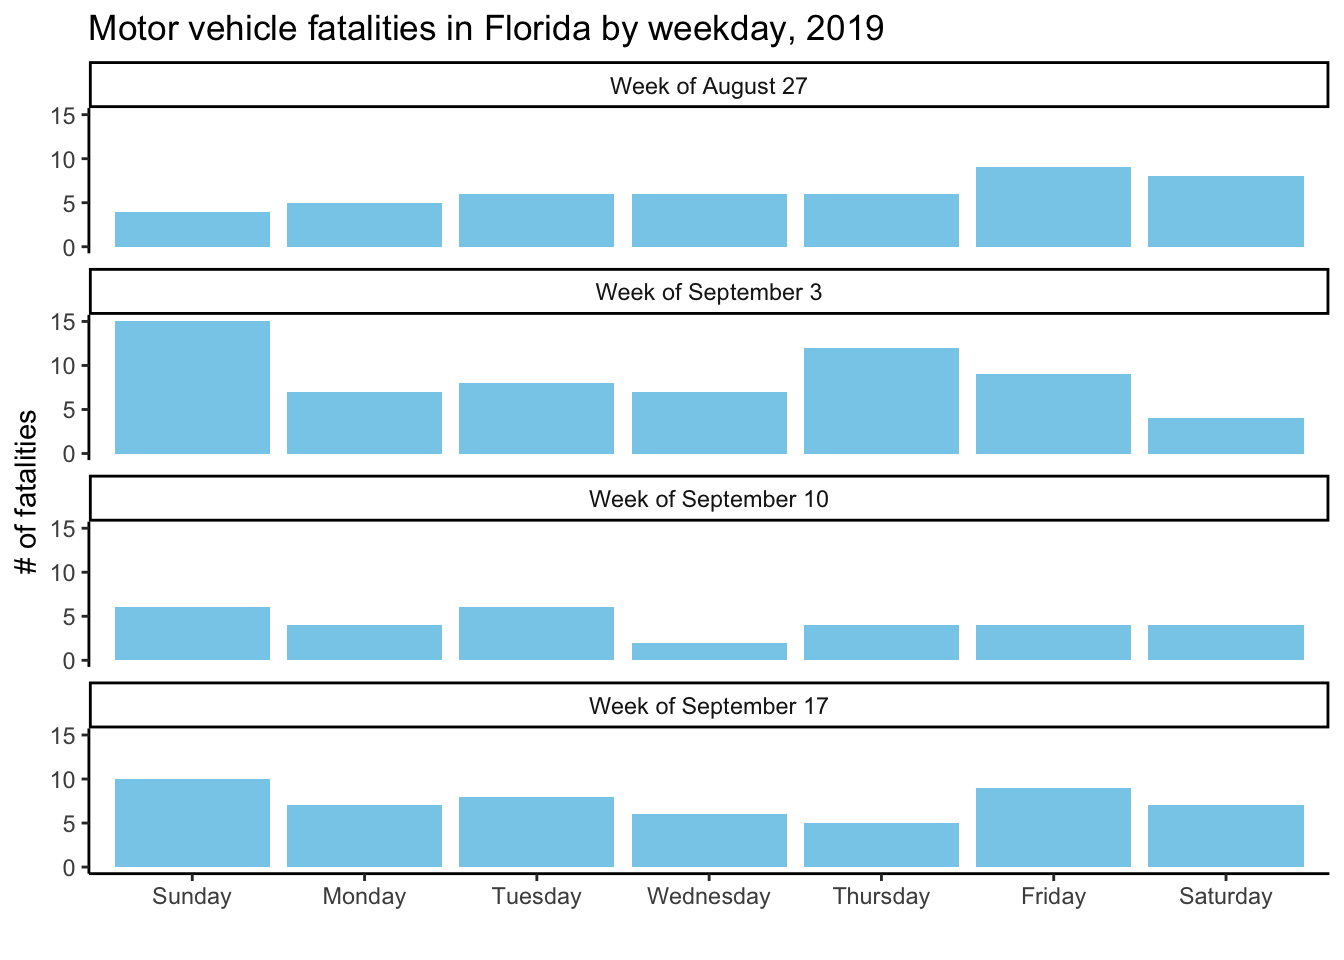
\includegraphics{navy_public_health_files/figure-latex/unnamed-chunk-9-1}

To save this plot to a file, you can use the \texttt{ggsave} function. This function can save
the plot in several different formats (e.g., pdf, jpeg, png, svg). Further, it allows you
to specify the size you'd like for the height and width of the plot as well as the plot
resolution.

The following call will save the \texttt{irma\_fatalities\_plot} to your working directory,
which should be the R project directory you're using for the examples if you followed the
set-up in ``Prerequisites''. It will save the file as a pdf that is 6 inches tall by 5 inches
wide.

\begin{Shaded}
\begin{Highlighting}[]
\KeywordTok{ggsave}\NormalTok{(irma_fatalities_plot, }\DataTypeTok{filename =} \StringTok{"irma_fatalities.pdf"}\NormalTok{, }
    \DataTypeTok{device =} \StringTok{"pdf"}\NormalTok{, }\DataTypeTok{height =} \DecValTok{6}\NormalTok{, }\DataTypeTok{width =} \DecValTok{5}\NormalTok{, }\DataTypeTok{units =} \StringTok{"in"}\NormalTok{)}
\end{Highlighting}
\end{Shaded}

\hypertarget{learn-more}{%
\section{Learn more}\label{learn-more}}

The \texttt{ggplot} framework has become extremely popular, and there are a lot of excellent
resources for learning more about how to use it. Many of these are through the website
\href{https://bookdown.org}{bookdown.org}, which hosts a collection of free, author-submitted
online books, mostly about R programming.

\href{https://r4ds.had.co.nz/}{R for Data Science} is a global look at effectively using
R's ``tidyverse'', including sections on plotting with \texttt{ggplot2}.
Kiernan Healy's \href{https://socviz.co/index.html\#preface}{Data Visualization: A Practical Introduction}
is a great book on using R for plotting, with extensive examples in R. This book also covers a lot
of the principles of creating effective and attractive plots---it's well worth reading.

If you want to dig deeper into plotting in R using the \texttt{ggplot} framework, you might want to
take a look at the official \texttt{ggplot2} book,
\href{https://www.amazon.com/ggplot2-Elegant-Graphics-Data-Analysis/dp/0387981403}{ggplot2: Elegant Graphics for Data Analysis} and
at Paul Murrell's book \href{https://www.amazon.com/Graphics-Third-Chapman-Hall-CRC/dp/1498789056/ref=sr_1_1?keywords=paul+murrell+r+graphics\&qid=1553696167\&s=books\&sr=1-1-spell}{R Graphics}, with
extensive coverage of the grid graphics system that \texttt{ggplot2} builds on.

Finally, one of the best ways to learn more is to check out RStudio's ``Data Visualization''
cheatsheet,\footnote{\textbf{cheatsheet.} A two-sided, one-page sheet crammed with all the main functions
  for a particular topic of coding. RStudio has a large collection available
  \href{https://www.rstudio.com/resources/cheatsheets/}{here}, including cheatsheets for cleaning
  data, working with factors and strings, and a range of other topics. This webpage also includes
  ``contributed'' cheatsheets, developed by people outside of RStudio.} Once you've started to
get the hang of the basics of plotting in R, download this cheatsheet and work through the
examples. All of them use datasets that come with R, so you should be able to run them all,
and you'll get a good idea of the range of plots \texttt{ggplot2} can be used to create.

\hypertarget{map}{%
\chapter{Map}\label{map}}

\newthought{R has had tools for mapping spatial} data for a long time, but some of these
tools, but they could take a while to learn if you were just used to basic plotting
in R. Recently, some packages have been developed for mapping spatial data that fit within
the \texttt{ggplot} framework, so they allow you to take what you've learned about creating non-geographical
plots and apply them to create maps.

The \texttt{sf} package \citep{R-sf} is a fantastic new(-ish) package for mapping in R. The ``Tidy'' section
of this handout describes the ``tidy'' data framework used as an input for \texttt{ggplot} code. The
``tidy'' data framework is also convenient for cleaning, merging, and manipulating data
before plotting or modeling it. The \texttt{sf} package allows you to read in and work with geographical
data in a tidy format. It turns out that this is very powerful, as you can learn how to do a
few things well (plotting {[}see the ``Plot'' section{]} and working with data {[}see the ``Tidy'' section{]}),
and then apply these tools in the same way, whether you're working with geographical or
non-geographical data.

\hypertarget{geographical-data-in-a-tidy-format}{%
\section{Geographical data in a tidy format}\label{geographical-data-in-a-tidy-format}}

The \texttt{sf} package allows you to create a dataframe object with one special characteristic: a
special \textbf{list column}\footnote{\textbf{list column}}
called ``geometry'' that contains the geometrical data needed to draw
an observation. For example, if you have a dataset of motor vehicle accidents, where each
row gives the data for an accident, the \texttt{geometry} column might include the latitude and
longitude for the location of the accident. As another example, if you have a data set of
the total number of motor vehicle fatalities in a year in each county in a state, the
\texttt{geometry} column might have all the latitude and longitude points to form the
boundary of each county.

These special dataframes are given a class called \textbf{sf}\footnote{\textbf{sf.} Short for ``simple features'',
  the name of both an R package and the object class created and used by the data. This class
  includes a special column called ``geometry'' for geographic information about each observation.
  Objects with this class can be used for mapping spatial data, but also can be manipulated
  using tidyverse tools very similarly to tibbles.}

There are several ways for you to create this special type of dataframe. We'll create a few
to use in the later mapping examples. First, if you have a regular dataframe, you can
convert it into an \texttt{sf} object, specifying which parts of the dataframe include geographical
information.

If you followed all the set-up instructions in the ``Prerequisites'', you should have downloaded a
dataset called ``fl\_accidents.csv'' and saved it in the ``data'' subdirectory of the R Project directory
for the examples. You can use \texttt{readr} to read it in. If you print out the start of it, you'll see
that it's got observations (rows) of fatal motor vehicle accidents. These accidents all occurred in
Florida within a week of Hurricane Irma's landfall on September 10, 2017. The columns give
the county code (\texttt{fips}), date (\texttt{date}), location (\texttt{latitude} and \texttt{longitud}), and the number of
fatalities (\texttt{fatals}).

\begin{Shaded}
\begin{Highlighting}[]
\KeywordTok{library}\NormalTok{(readr)}
\NormalTok{fl_accidents <-}\StringTok{ }\KeywordTok{read_csv}\NormalTok{(}\StringTok{"data/fl_accidents.csv"}\NormalTok{)}
\end{Highlighting}
\end{Shaded}

\begin{verbatim}
## Parsed with column specification:
## cols(
##   fips = col_double(),
##   date = col_date(format = ""),
##   latitude = col_double(),
##   longitud = col_double(),
##   fatals = col_double()
## )
\end{verbatim}

\begin{Shaded}
\begin{Highlighting}[]
\NormalTok{fl_accidents}
\end{Highlighting}
\end{Shaded}

\begin{verbatim}
## # A tibble: 37 x 5
##     fips date       latitude longitud fatals
##    <dbl> <date>        <dbl>    <dbl>  <dbl>
##  1 12031 2017-09-08     30.2    -81.5      1
##  2 12095 2017-09-07     28.5    -81.4      1
##  3 12097 2017-09-08     28.3    -81.3      1
##  4 12095 2017-09-07     28.6    -81.2      1
##  5 12031 2017-09-08     30.2    -81.8      1
##  6 12033 2017-09-07     30.6    -87.4      2
##  7 12023 2017-09-10     30.1    -82.7      1
##  8 12075 2017-09-08     29.6    -82.9      1
##  9 12045 2017-09-09     30.1    -85.3      2
## 10 12031 2017-09-12     30.4    -81.8      1
## # ... with 27 more rows
\end{verbatim}

Even though this data has geographical information in it (latitude and longitude), it's currently
just a regular dataframe. To convert it to an \texttt{sf} class object, you can use the \texttt{st\_as\_sf} function,\footnote{Most of the functions in the \texttt{st} package start with \texttt{st\_}. Since R studio allows \textbf{tab completion},
  this makes it very easy to look up a function in the package whose name you might have forgotten.
  Just try typing \texttt{st\_} and then the Tab key in your R console---you should get a pop-up with a list of
  suggestions for possible function names.}
specifying the columns with the geogrphical coordinates using the \texttt{coords} parameter.\footnote{Here, the
  compound pipe operator, \texttt{\%\textless{}\textgreater{}\%}, applies the function to \texttt{fl\_accidents} and then overwrites the
  \texttt{fl\_accidents} with the modified version, updating the object so you're ready to use it for later
  code.}

\begin{Shaded}
\begin{Highlighting}[]
\KeywordTok{library}\NormalTok{(sf)}
\NormalTok{fl_accidents }\OperatorTok\StringTok{ }\KeywordTok{st_as_sf}\NormalTok{(}\DataTypeTok{coords =} \KeywordTok{c}\NormalTok{(}\StringTok{"longitud"}\NormalTok{, }
    \StringTok{"latitude"}\NormalTok{))}
\end{Highlighting}
\end{Shaded}

Now, when you print out \texttt{fl\_accidents}, you'll see some extra information at the top of the print
out, including the objects \textbf{bounding box} (\texttt{bbox}) and \textbf{projection} (\texttt{epsg}, \texttt{proj4string})
(which we currently haven't set).

\begin{Shaded}
\begin{Highlighting}[]
\NormalTok{fl_accidents}
\end{Highlighting}
\end{Shaded}

\begin{verbatim}
## Simple feature collection with 37 features and 3 fields
## geometry type:  POINT
## dimension:      XY
## bbox:           xmin: -87.3797 ymin: 25.6876 xmax: -80.32332 ymax: 30.65894
## epsg (SRID):    NA
## proj4string:    NA
## # A tibble: 37 x 4
##     fips date       fatals
##    <dbl> <date>      <dbl>
##  1 12031 2017-09-08      1
##  2 12095 2017-09-07      1
##  3 12097 2017-09-08      1
##  4 12095 2017-09-07      1
##  5 12031 2017-09-08      1
##  6 12033 2017-09-07      2
##  7 12023 2017-09-10      1
##  8 12075 2017-09-08      1
##  9 12045 2017-09-09      2
## 10 12031 2017-09-12      1
## # ... with 27 more rows, and 1 more
## #   variable: geometry <POINT>
\end{verbatim}

A second way to create an \texttt{sf} object in R is to read in data from a geographic data file, like
a \textbf{shapefile}\footnote{\textbf{shapefile.} \ldots{}}
If you followed the ``Prerequisites'', you should have downloaded a file called
``al112017\_best\_track.zip''. This is a zipped file that includes shapefiles for the track of
Hurricane Irma from the National Hurricane Center ({[}website{]}).

First, you'll need to unzip this file to ``unpack'' it as a directory of files. On many
computers, you can do this by double-clicking on the zipped file. However, you can also
unzip files from R. Just run:

\begin{Shaded}
\begin{Highlighting}[]
\KeywordTok{unzip}\NormalTok{(}\StringTok{"data/al112017_best_track.zip"}\NormalTok{, }\DataTypeTok{exdir =} \StringTok{"data/al112017_best_track"}\NormalTok{)}
\end{Highlighting}
\end{Shaded}

Once the file is unzipped, if you look at the ``al112017\_best\_track'' directory created,
you will see that it contains a collection of files starting with one of several roots
(e.g., ``al112017\_lin'') and with one of several suffixes (e.g., ``.dbf'', ``.prj'', ``.shx'').

\begin{Shaded}
\begin{Highlighting}[]
\KeywordTok{list.files}\NormalTok{(}\StringTok{"data/al112017_best_track/"}\NormalTok{)}
\end{Highlighting}
\end{Shaded}

\begin{verbatim}
##  [1] "al112017_lin.dbf"          
##  [2] "al112017_lin.prj"          
##  [3] "al112017_lin.shp"          
##  [4] "al112017_lin.shp.xml"      
##  [5] "al112017_lin.shx"          
##  [6] "al112017_pts.dbf"          
##  [7] "al112017_pts.prj"          
##  [8] "al112017_pts.shp"          
##  [9] "al112017_pts.shp.xml"      
## [10] "al112017_pts.shx"          
## [11] "al112017_radii.dbf"        
## [12] "al112017_radii.prj"        
## [13] "al112017_radii.shp"        
## [14] "al112017_radii.shp.xml"    
## [15] "al112017_radii.shx"        
## [16] "al112017_windswath.dbf"    
## [17] "al112017_windswath.prj"    
## [18] "al112017_windswath.shp"    
## [19] "al112017_windswath.shp.xml"
## [20] "al112017_windswath.shx"
\end{verbatim}

Each set of files with the same root provides a ``layer'' of the shapefile, giving a set
of geographic information. For example, the ``al112017\_lin.\emph{" files provides the
line of the hurricane's track, while the "al112017\_windswarth.}'' layer provides windswaths
(how severe the wind was in certain locations surrounding the storm track).

You can read in any of these layers into R as an \texttt{sf} object using \texttt{irma\_tracks} and specifying
the layer you'd like from the directory with the \texttt{layer} parameter (put the root of the filenames
for the layer you want). For example, to read in a line with the track of irma, you can run:

\begin{Shaded}
\begin{Highlighting}[]
\NormalTok{irma_tracks <-}\StringTok{ }\KeywordTok{st_read}\NormalTok{(}\StringTok{"data/al112017_best_track/"}\NormalTok{, }
    \DataTypeTok{layer =} \StringTok{"al112017_lin"}\NormalTok{)}
\end{Highlighting}
\end{Shaded}

\begin{verbatim}
## Reading layer `al112017_lin' from data source `/Users/georgianaanderson/Documents/r_workshops/navy_public_health/data/al112017_best_track' using driver `ESRI Shapefile'
## Simple feature collection with 20 features and 3 fields
## geometry type:  LINESTRING
## dimension:      XY
## bbox:           xmin: -90.1 ymin: 16.1 xmax: -26.9 ymax: 36.8
## epsg (SRID):    NA
## proj4string:    +proj=longlat +a=6371200 +b=6371200 +no_defs
\end{verbatim}

If you print out \texttt{irma\_tracks}, you can see that it looks like a dataframe, but with extra
geographic information (bounding box, projection, etc.) as well as a special column for
geometry, which gives the latitude and longitude \ldots{}

\begin{Shaded}
\begin{Highlighting}[]
\NormalTok{irma_tracks}
\end{Highlighting}
\end{Shaded}

\begin{verbatim}
## Simple feature collection with 20 features and 3 fields
## geometry type:  LINESTRING
## dimension:      XY
## bbox:           xmin: -90.1 ymin: 16.1 xmax: -26.9 ymax: 36.8
## epsg (SRID):    NA
## proj4string:    +proj=longlat +a=6371200 +b=6371200 +no_defs
## First 10 features:
##    STORMNUM           STORMTYPE SS
## 1        11 Tropical Depression  0
## 2        11      Tropical Storm  0
## 3        11          Hurricane1  1
## 4        11          Hurricane2  2
## 5        11          Hurricane3  3
## 6        11          Hurricane2  2
## 7        11          Hurricane3  3
## 8        11          Hurricane4  4
## 9        11          Hurricane5  5
## 10       11          Hurricane4  4
##                          geometry
## 1  LINESTRING (-26.9 16.1, -28...
## 2  LINESTRING (-28.3 16.2, -29...
## 3  LINESTRING (-32.5 16.4, -33...
## 4  LINESTRING (-34.2 17.1, -35...
## 5  LINESTRING (-35.1 17.5, -36...
## 6  LINESTRING (-42.6 18.9, -44...
## 7  LINESTRING (-47.9 17.9, -49...
## 8  LINESTRING (-53.9 16.7, -55...
## 9  LINESTRING (-57.8 16.7, -59...
## 10 LINESTRING (-73 21.5, -73.2...
\end{verbatim}

\hypertarget{basic-mapping}{%
\section{Basic mapping}\label{basic-mapping}}

\begin{Shaded}
\begin{Highlighting}[]
\KeywordTok{library}\NormalTok{(ggplot2)}

\KeywordTok{ggplot}\NormalTok{() }\OperatorTok{+}\StringTok{ }\KeywordTok{geom_sf}\NormalTok{(}\DataTypeTok{data =}\NormalTok{ fl_accidents)}
\end{Highlighting}
\end{Shaded}

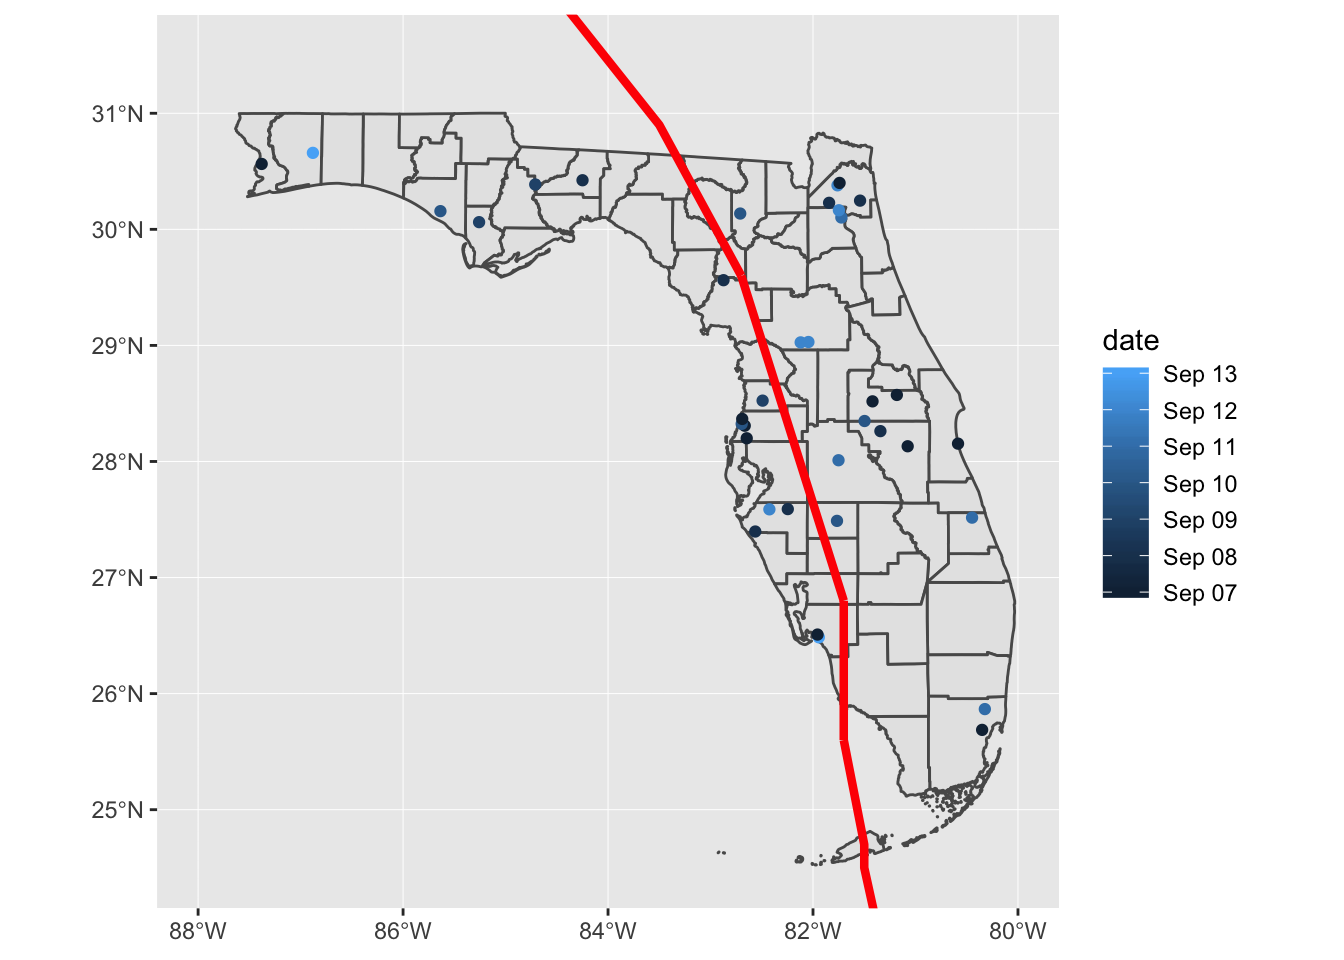
\includegraphics{navy_public_health_files/figure-latex/unnamed-chunk-18-1}

\hypertarget{learn-more-1}{%
\section{Learn more}\label{learn-more-1}}

The \texttt{sf} package is rapidly developing, and so it is worthwhile to seek out the latest
help guides and tutorials to learn more about the system, particularly if you are doing
this a while after the spring 2019 workshop.

The package authors have created
\href{https://cran.r-project.org/web/packages/sf/vignettes/sf1.html}{a website with more on the package}.
They also have a book called \href{https://geocompr.robinlovelace.net/}{Geocomputation with R}, which
is currently available online and will be available in print sometime in 2019.

Both these sources go in depth to describe the \texttt{sf} package and how to use it. If you want
other examples of using the package, many people have recently written blog posts with examples
of using it, so it's worth googling something like ``blog post map r sf''.

\hypertarget{interact}{%
\chapter{Interact}\label{interact}}

\hypertarget{dt-datatables}{%
\section{DT: Datatables}\label{dt-datatables}}

\begin{Shaded}
\begin{Highlighting}[]
\KeywordTok{library}\NormalTok{(readr)}
\KeywordTok{library}\NormalTok{(dplyr)}
\KeywordTok{library}\NormalTok{(sf)}
\NormalTok{fl_accidents <-}\StringTok{ }\KeywordTok{read_csv}\NormalTok{(}\StringTok{"data/fl_accidents.csv"}\NormalTok{)}
\end{Highlighting}
\end{Shaded}

\begin{Shaded}
\begin{Highlighting}[]
\KeywordTok{library}\NormalTok{(DT)}
\KeywordTok{datatable}\NormalTok{(fl_accidents)}
\end{Highlighting}
\end{Shaded}

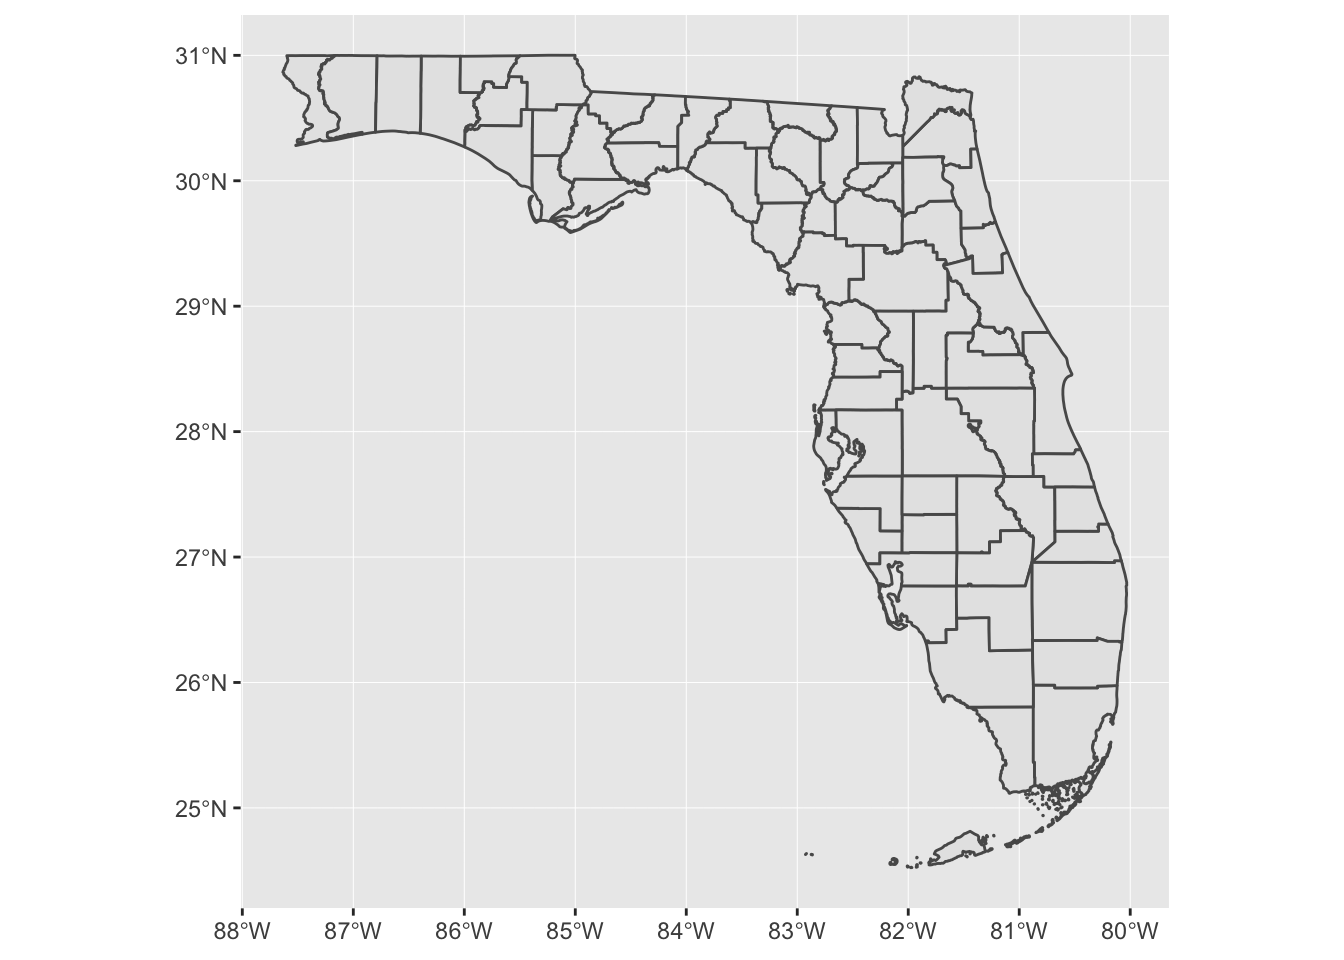
\includegraphics{navy_public_health_files/figure-latex/unnamed-chunk-20-1}

\begin{Shaded}
\begin{Highlighting}[]
\KeywordTok{datatable}\NormalTok{(fl_accidents, }\DataTypeTok{class =} \StringTok{"compact"}\NormalTok{, }\DataTypeTok{caption =} \StringTok{"Fatal motor vehicle accidents in Florida the week of Hurricane Irma"}\NormalTok{, }
    \DataTypeTok{colnames =} \KeywordTok{c}\NormalTok{(}\StringTok{"County FIPS"}\NormalTok{, }\StringTok{"Date"}\NormalTok{, }\StringTok{"Latitude"}\NormalTok{, }
        \StringTok{"Longitude"}\NormalTok{, }\StringTok{"# fatalities"}\NormalTok{))}
\end{Highlighting}
\end{Shaded}

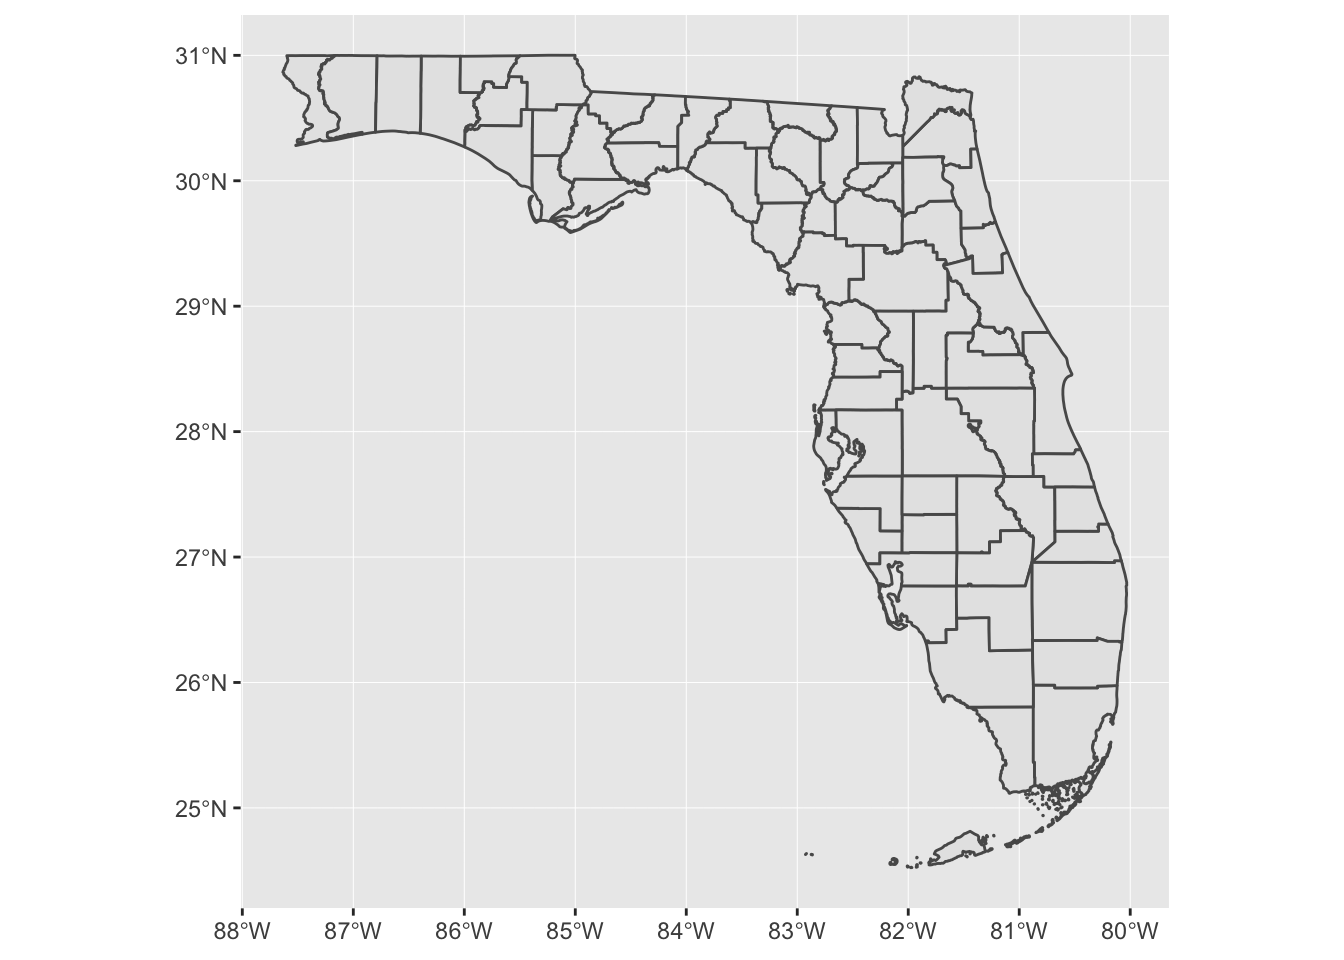
\includegraphics{navy_public_health_files/figure-latex/unnamed-chunk-21-1}

\hypertarget{plotly}{%
\section{Plotly}\label{plotly}}

\hypertarget{leaflet}{%
\section{Leaflet}\label{leaflet}}

\begin{Shaded}
\begin{Highlighting}[]
\KeywordTok{library}\NormalTok{(magrittr)}
\KeywordTok{library}\NormalTok{(leaflet)}
\NormalTok{fl_accidents }\OperatorTok\StringTok{ }\KeywordTok{st_as_sf}\NormalTok{(}\DataTypeTok{coords =} \KeywordTok{c}\NormalTok{(}\StringTok{"longitud"}\NormalTok{, }
    \StringTok{"latitude"}\NormalTok{))}
\KeywordTok{leaflet}\NormalTok{() }\OperatorTok\StringTok{ }\KeywordTok{addTiles}\NormalTok{() }\OperatorTok\StringTok{ }\KeywordTok{addMarkers}\NormalTok{(}\DataTypeTok{data =}\NormalTok{ fl_accidents)}
\end{Highlighting}
\end{Shaded}

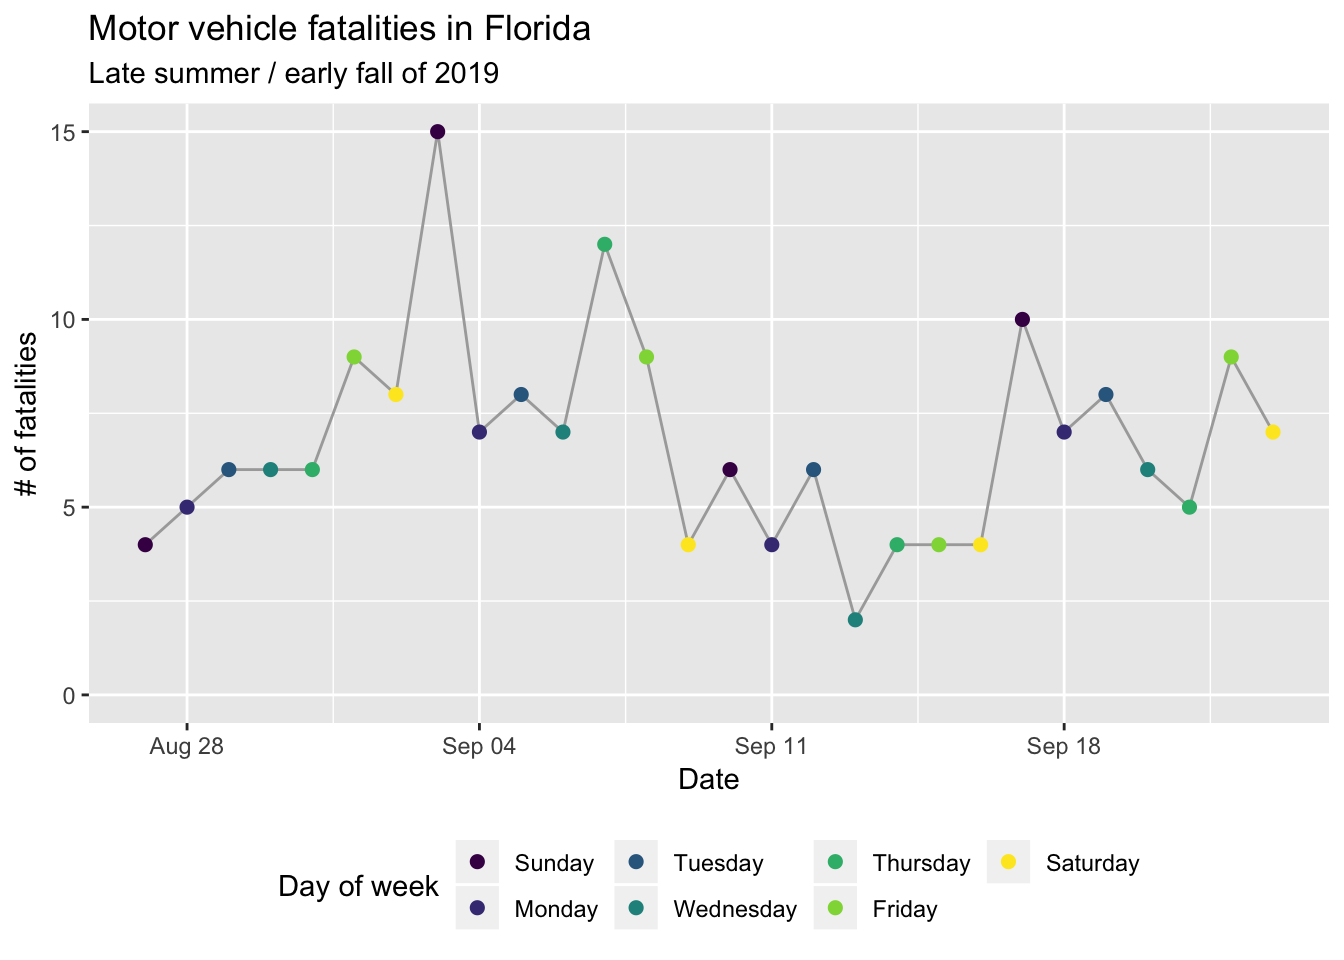
\includegraphics{navy_public_health_files/figure-latex/unnamed-chunk-22-1}

\hypertarget{learn-more-2}{%
\section{Learn more}\label{learn-more-2}}

\hypertarget{report}{%
\chapter{Report}\label{report}}

\hypertarget{rmarkdown}{%
\section{RMarkdown}\label{rmarkdown}}

\hypertarget{dashboards}{%
\section{Dashboards}\label{dashboards}}

\hypertarget{tidy}{%
\chapter{Tidy}\label{tidy}}

\newthought{The **ggplot2** framework is a} very efficient and powerful
framework for
creating visualizations. This comes in part from the fact that it sticks
to a specific data format for its input. It requires you to start with
data in a what's called a ``tidy'' format.

In the previous section, I used an example dataset that was already in this
format, to make it easier for you to get started with plotting. However,
to leverage the power of \textbf{ggplot2} for real datasets, you have to know
how to get them into this tidy format. This section will explain this format,
as well as how you can clean real datasets to convert them into this format.

\hypertarget{tidy-format}{%
\section{Tidy format}\label{tidy-format}}

\newthought{When you hear the term} ``tidy data'', you might just think of a ``clean''
dataset---one where unneeded columns have been removed, for example, and
perhaps that's in a nice \textbf{rectangular format}.\footnote{\textbf{rectangular format.} A data format
  where each column has data in the same class (e.g., date, number) and is the
  same length. (Think of the format of data in a table of a paper, or in a clean
  Excel spreadsheet.}

{[}More about tidy data{]}

\hypertarget{tidyverse-tools}{%
\section{Tidyverse tools}\label{tidyverse-tools}}

\newthought{As an epidemiologist,} I meet many people who learned SAS as students
and continue
to use it. A common misperception is that R is good for visualizations, but bad for
cleaning data. While in the past this might have been (somewhat) valid, now it couldn't
be further from the truth. With a collection of tools available through the
\textbf{tidyverse},\footnote{\textbf{tidyverse.} A collection of packages to work with data in a
  ``tidy'' format, or to convert it to that format if needed. Many of these packages
  are developed and maintained by people at RStudio. If you run \texttt{library("tidyverse")},
  you can load the core tidyverse packages in your R session. This way, you avoid
  having to load them one by one.}
you can write clean and compact code to clean even very large and
messy datasets.

This collection of tools follows the principle that hard problems can be best solved
by small tools that can be combined together, very much in-line with the \textbf{Unix
philosophy}.

The tidyverse works as well as it does because, for many parts of it, it requires
a common input and output, and those input and output specifications are
identical (the tidy data format).
If you want to get a better idea of this concept, and why it's so powerful,
think of some of the
classic toys, like Legos (train sets and Lincoln logs also
work here). Each piece takes the same input and produces the same output. Think of
the bottom of a Lego---it ``inputs'' small, regularly-spaced pegs, which are exactly
what's at the top (``output'') of each Lego block. This common input and output
means that the blocks can be joined together in an extraordinary number of
different combinations, and that you can imagine and then make very complex
structures with the blocks.

\hypertarget{subsetting}{%
\section{Subsetting}\label{subsetting}}

\hypertarget{selecting-columns}{%
\subsection{Selecting columns}\label{selecting-columns}}

\hypertarget{slicing-rows}{%
\subsection{Slicing rows}\label{slicing-rows}}

\hypertarget{filtering-rows}{%
\subsection{Filtering rows}\label{filtering-rows}}

\hypertarget{adding}{%
\section{Adding}\label{adding}}

\hypertarget{summarizing}{%
\section{Summarizing}\label{summarizing}}

\hypertarget{reformatting}{%
\section{Reformatting}\label{reformatting}}

\hypertarget{final-words}{%
\chapter{Final Words}\label{final-words}}

We have finished a nice book.

\bibliography{book.bib,packages.bib}



\end{document}
